\PassOptionsToPackage{unicode=true}{hyperref} % options for packages loaded elsewhere
\PassOptionsToPackage{hyphens}{url}
\documentclass[11pt,dvipsnames,ignorenonframetext,aspectratio=169]{beamer}
\IfFileExists{pgfpages.sty}{\usepackage{pgfpages}}{}
\setbeamertemplate{caption}[numbered]
\setbeamertemplate{caption label separator}{: }
\setbeamercolor{caption name}{fg=normal text.fg}
\beamertemplatenavigationsymbolsempty
\usepackage{lmodern}
\usepackage{amssymb,amsmath}
\usepackage{ifxetex,ifluatex}
\usepackage{fixltx2e} % provides \textsubscript
\ifnum 0\ifxetex 1\fi\ifluatex 1\fi=0 % if pdftex
  \usepackage[T1]{fontenc}
  \usepackage[utf8]{inputenc}
\else % if luatex or xelatex
  \ifxetex
    \usepackage{mathspec}
  \else
    \usepackage{fontspec}
\fi
\defaultfontfeatures{Ligatures=TeX,Scale=MatchLowercase}







\fi

  \usetheme[]{monash}

  \usecolortheme{monashwhite}


% A default size of 24 is set in beamerthememonash.sty
  \setbeamerfont{title}{series=\bfseries,parent=structure,size=\fontsize{18pt}{32}}

% Title page
\setbeamertemplate{title page}
{\placefig{-0.01}{-0.01}{width=1.01\paperwidth,height=1.01\paperheight}{barleyfloret.jpg}
\begin{textblock}{7.5}(1,2.8)\usebeamerfont{title}
{\color{white}\raggedright\par\inserttitle}
\end{textblock}
\begin{textblock}{7.5}(1,7)
{\color{white}\raggedright{\insertauthor}\mbox{}\\[0.2cm]
\insertdate}
\end{textblock}}


  \useinnertheme{rounded}

  \useoutertheme{smoothtree}

% use upquote if available, for straight quotes in verbatim environments
\IfFileExists{upquote.sty}{\usepackage{upquote}}{}
% use microtype if available
\IfFileExists{microtype.sty}{%
  \usepackage{microtype}
  \UseMicrotypeSet[protrusion]{basicmath} % disable protrusion for tt fonts
}{}


\newif\ifbibliography
  \usepackage[round]{natbib}
  \bibliographystyle{plainnat}


\hypersetup{
      pdftitle={The nature of gene},
            colorlinks=true,
    linkcolor=red,
    citecolor=Blue,
    urlcolor=lightgrayd,
    breaklinks=true}
%\urlstyle{same}  % Use monospace font for urls







% Prevent slide breaks in the middle of a paragraph:
\widowpenalties 1 10000
\raggedbottom

  \AtBeginPart{
    \let\insertpartnumber\relax
    \let\partname\relax
    \frame{\partpage}
  }
  \AtBeginSection{
    \ifbibliography
    \else
      \let\insertsectionnumber\relax
      \let\sectionname\relax
      \frame{\sectionpage}
    \fi
  }
  \AtBeginSubsection{
    \let\insertsubsectionnumber\relax
    \let\subsectionname\relax
    \frame{\subsectionpage}
  }



\setlength{\parindent}{0pt}
\setlength{\parskip}{6pt plus 2pt minus 1pt}
\setlength{\emergencystretch}{3em}  % prevent overfull lines
\providecommand{\tightlist}{%
  \setlength{\itemsep}{0pt}\setlength{\parskip}{0pt}}

  \setcounter{secnumdepth}{0}


%% Monash overrides
\AtBeginSection[]{
   \frame<beamer>{
   \frametitle{Outline}\vspace*{0.2cm}
   
   \tableofcontents[currentsection,hideallsubsections]
  }}

% Redefine shaded environment if it exists (to ensure text is black)
\ifcsname Shaded\endcsname
  \definecolor{shadecolor}{RGB}{225,225,225}
  \renewenvironment{Shaded}{\color{black}\begin{snugshade}\color{black}}{\end{snugshade}}
\fi
%%

  \usepackage{setspace}
  \usepackage{wasysym}
  % \usepackage{footnote} % don't use this this breaks all
  \usepackage{fontenc}
  \usepackage{fontawesome}
  \usepackage{booktabs,siunitx}
  \usepackage{longtable}
  \usepackage{array}
  \usepackage{multirow}
  \usepackage{wrapfig}
  \usepackage{float}
  \usepackage{colortbl}
  \usepackage{pdflscape}
  \usepackage{tabu}
  \usepackage{threeparttable}
  \usepackage{threeparttablex}
  \usepackage[normalem]{ulem}
  \usepackage{makecell}
  \usepackage{xcolor}
  \usepackage{tikz} % required for image opacity change
  \usepackage[absolute,overlay]{textpos} % for text formatting
  \usepackage{chemfig}
  \usepackage[skip=0.333\baselineskip]{caption}
  % \newcommand*{\AlignChar}[1]{\makebox[1ex][c]{\ensuremath{\scriptstyle#1}}}%

  % this font option is amenable for beamer
  \setbeamerfont{caption}{size=\tiny}
  \singlespacing
  \definecolor{lightgrayd}{gray}{0.95}
  \definecolor{skyblued}{rgb}{0.65, 0.6, 0.94}
  \definecolor{oranged}{RGB}{245, 145, 200}

  % \newlength{\cslhangindent}
  % \setlength{\cslhangindent}{1.5em}
  % \newenvironment{cslreferences}%
  %   {\setlength{\parindent}{0pt}%
  %   \everypar{\setlength{\hangindent}{\cslhangindent}}\ignorespaces}%
  %   {\par}
    
  \newlength{\cslhangindent}
  \setlength{\cslhangindent}{1.5em}
  \newenvironment{CSLReferences}%
  {\setlength{\parindent}{0pt}%
  \everypar{\setlength{\hangindent}{\cslhangindent}}\ignorespaces}%
  {\par}

  \newcommand{\bcolumns}{\begin{columns}[T, onlytextwidth]}
  \newcommand{\ecolumns}{\end{columns}}

  \newcommand{\bdescription}{\begin{description}}
  \newcommand{\edescription}{\end{description}}

  \newcommand{\bitemize}{\begin{itemize}}
  \newcommand{\eitemize}{\end{itemize}}
  \AtBeginSubsection{}

  \title[]{The nature of gene}


  \author[
        Deependra Dhakal\\
Agriculture and Forestry University\\
\textit{ddhakal.rookie@gmail.com}\\
\url{https://rookie.rbind.io}
    ]{Deependra Dhakal\\
Agriculture and Forestry University\\
\textit{ddhakal.rookie@gmail.com}\\
\url{https://rookie.rbind.io}}


\date[
      
  ]{
    }

\begin{document}

% Hide progress bar and footline on titlepage
  \begin{frame}[plain]
  \titlepage
  \end{frame}


   \frame<beamer>{
   \frametitle{Outline}\vspace*{0.2cm}
   
   \tableofcontents[hideallsubsections]
  }

\hypertarget{gene}{%
\section{Gene}\label{gene}}

\begin{frame}{Genetic analysis begins with mutants}
\protect\hypertarget{genetic-analysis-begins-with-mutants}{}
\begin{itemize}
\tightlist
\item
  Genetic approach to understanding any biological property is through
  gene discovery
\item
  One simple and useful analytical approaches to gene discovery is
  detection of single-gene inheritance pattern.
\item
  Variants in biological system represent ``tweaks'' in the biological
  machine.
\item
  Common form of any property of an organism is called \textbf{wild
  type}
\item
  Heritable variants different from wild types are called
  \textbf{mutants}
\item
  Alternative forms of the property are called \textbf{phenotypes}
\item
  \textbf{Polymorphism}: coexistence of two or more reasonably common
  phenotypes of a biological property
\end{itemize}
\end{frame}

\begin{frame}{Approaches to gene identification}
\protect\hypertarget{approaches-to-gene-identification}{}
\bcolumns
\column{0.5\textwidth}

\begin{itemize}
\tightlist
\item
  This type of approach to gene discovery is sometimes called
  \textbf{forward genetics}, a strategy to understanding biological
  function starting with random single-gene mutants and ending with
  their DNA sequence and biochemical function.
\item
  \textbf{Reverse genetics} starts with genomic analysis at the DNA
  level to identify a set of genes as candidates for encoding the
  biological property of
  interest\footnote[frame]{For a book chapter dedicated to Reverse genetics approaches, refer to \cite{gilchrist2013gene}.}.
\end{itemize}

\column{0.5\textwidth}

\begin{figure}
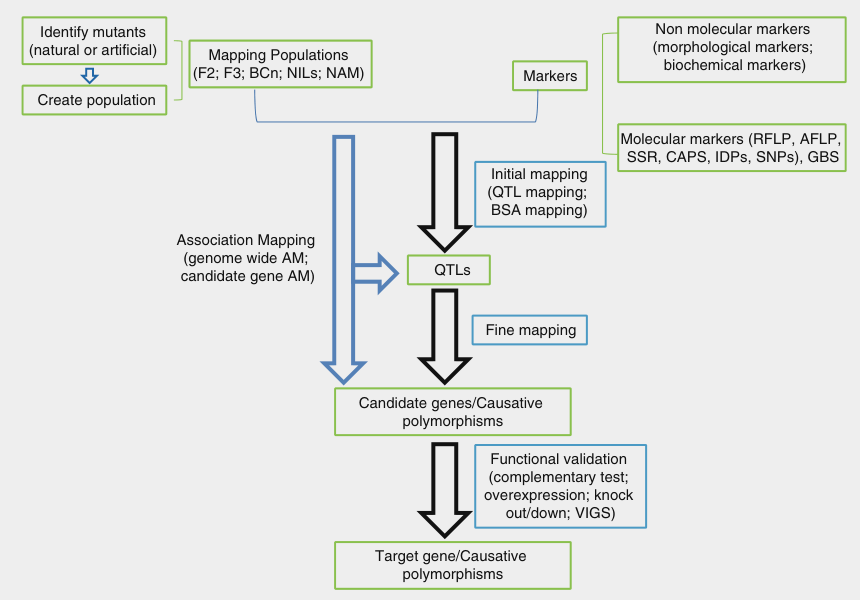
\includegraphics[width=0.8\linewidth]{../images/gene_id_forward_genetics} \caption{Flowchart of forward genetics approach in gene identification. For an entire chapter dedicated to the approach, refer to \cite{ji2013gene}}\label{fig:forward-genetics}
\end{figure}

\ecolumns
\end{frame}

\hypertarget{nature-of-genetic-code}{%
\section{Nature of genetic code}\label{nature-of-genetic-code}}

\begin{frame}{Physical nature}
\protect\hypertarget{physical-nature}{}
\begin{itemize}
\tightlist
\item
  Are genes composed of protein, nucleic acid, or some other substance?
\item
  In 1944, Oswald Avery, Colin MacLeod, and Maclyn McCarty offered the
  first compelling experimental evidence that genes are made of
  deoxyribonucleic acid (DNA).
\item
  They showed that DNA extracted from a virulent strain of bacteria
  carried the necessary genetic information to transform a nonvirulent
  strain into a virulent one.
\end{itemize}
\end{frame}

\begin{frame}{How can DNA molecules store information ?}
\protect\hypertarget{how-can-dna-molecules-store-information}{}
\begin{itemize}
\tightlist
\item
  In the 1950s, there was something of a race among several groups of
  geneticists and chemists to answer this question. In 1953, James
  Watson and Francis Crick working at Cambridge University in England
  won that race.
\item
  They determined that the molecular structure of DNA was in the form of
  a double helix -- two strands of DNA wound side-by-side in a spiral.
  Their structure of the double helix is like a twisted ladder (Figure
  \ref{fig:twisted-ladder}).
\item
  The sides of the ladder are made of sugar and phosphate groups. The
  rungs of the ladder are made of four bases: adenine (A), thymine (T),
  guanine (G), and cytosine (C).
\end{itemize}
\end{frame}

\begin{frame}{}
\protect\hypertarget{section}{}
\begin{itemize}
\tightlist
\item
  The bases face the center, and each base is hydrogen bonded to the
  base facing it in the opposite strand.
\item
  Nucleotide base pairing is highly specific. The bonding specificity is
  based on the complementary shapes and charges of the bases.
\item
  The sequence of A, T, G, and C represents the coded information
  carried by the DNA molecule.
\end{itemize}

\begin{figure}

{\centering 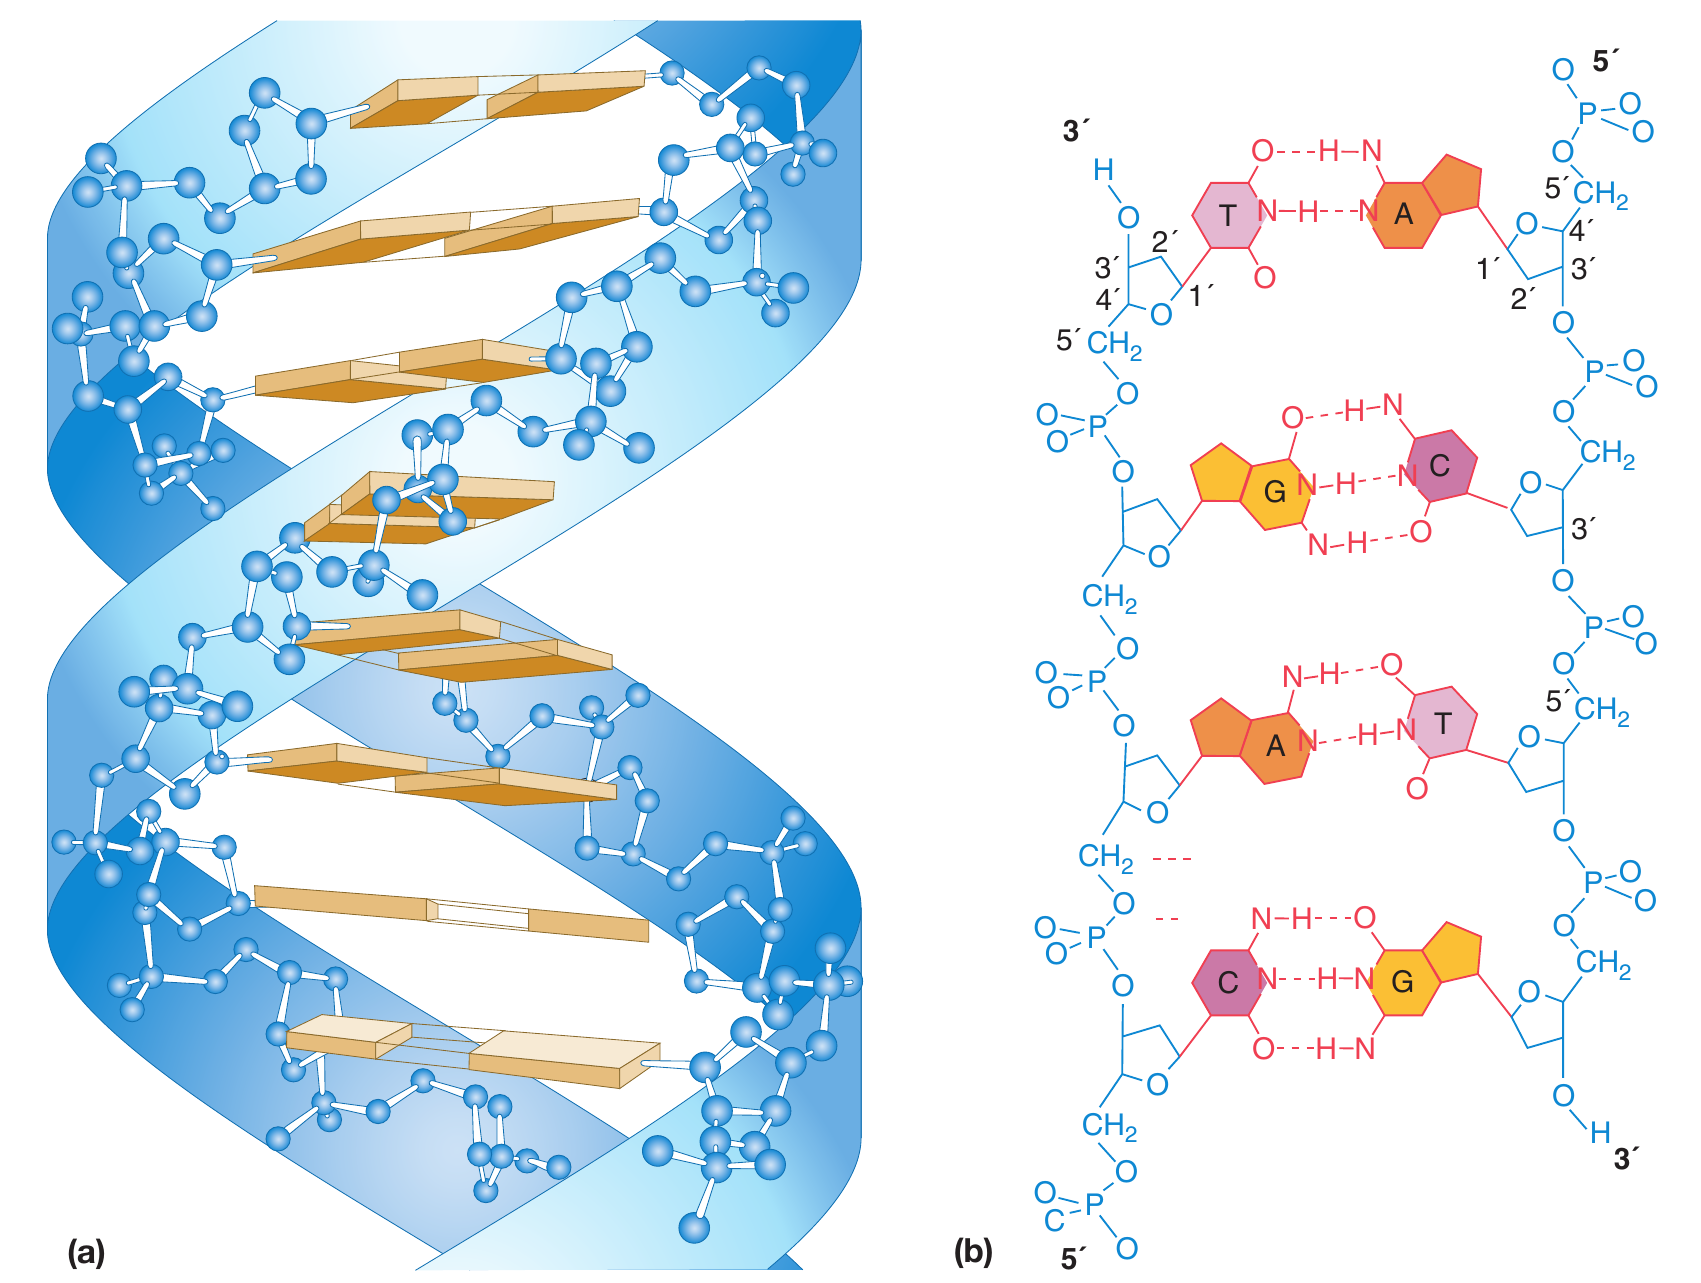
\includegraphics[width=0.38\linewidth]{../images/twisted_ladder_dna} 

}

\caption{Twisted ladder structure of DNA}\label{fig:twisted-ladder}
\end{figure}
\end{frame}

\begin{frame}{How are genes regulated?}
\protect\hypertarget{how-are-genes-regulated}{}
\begin{itemize}
\tightlist
\item
  Cells need mechanisms to turn genes on or off in specific cell and
  tissue types and at specific times during development.
\item
  In 1961, Francois Jacob and Jacques Monod made a conceptual
  breakthrough on this question.
\item
  Working the genes necessary to metabolize the sugar lactose in the
  bacterium \emph{Escherichia coli}, they demonstrated that genes have
  regulatory elements that regulate gene expression -- that is, whether
  a gene is turned on or off.
\item
  The regulatory elements are specific DNA sequences to which a
  regulatory protein binds and acts as either an activator or repressor
  of the expression of the gene.
\end{itemize}
\end{frame}

\begin{frame}{How is the information stored in DNA decoded to synthesize
protein ?}
\protect\hypertarget{how-is-the-information-stored-in-dna-decoded-to-synthesize-protein}{}
\begin{itemize}
\tightlist
\item
  While the discovery of the double-helical structure of DNA was a
  watershed for biology, many details were still unknown.
\item
  Precisely how information was encoded into DNA and how it was decoded
  to form the enzymes that Tatum and Beadle had shown to be the
  workhorses of gene action remained unknown.
\item
  Over the years 1961 through 1967, teams of molecular geneticists and
  chemists working in several countries answered these questions when
  they ``cracked the genetic code.''
\end{itemize}
\end{frame}

\begin{frame}{}
\protect\hypertarget{section-1}{}
\begin{itemize}
\tightlist
\item
  What this means is that they deduced how a string of DNA nucleotides,
  each with one of four different bases (A, T, C, or G), encodes the set
  of 20 different amino acids that are the building blocks of proteins.
\item
  They also discovered that there is a messenger molecule made of
  ribonucleic acid (RNA) that carries information in the DNA in the
  nucleus to the cytoplasm where proteins are synthesized.
\item
  By 1967, the basic flowchart for information transmission -- central
  dogma of biology -- in cells was known.
\end{itemize}
\end{frame}

\begin{frame}{Central dogma of biology}
\protect\hypertarget{central-dogma-of-biology}{}
\bcolumns
\column{0.6\textwidth}

\begin{itemize}
\tightlist
\item
  The flow of genetic information in cells from DNA to mRNA to protein
  is described by the Central Dogma.
\item
  The decoding of one molecule to another is performed by specific
  proteins and RNAs.
\item
  Because the information stored in DNA is so central to cellular
  function, it makes sense that the cell would make mRNA copies of this
  information for protein synthesis, while keeping the DNA itself intact
  and protected.
\end{itemize}

\column{0.4\textwidth}

\begin{figure}
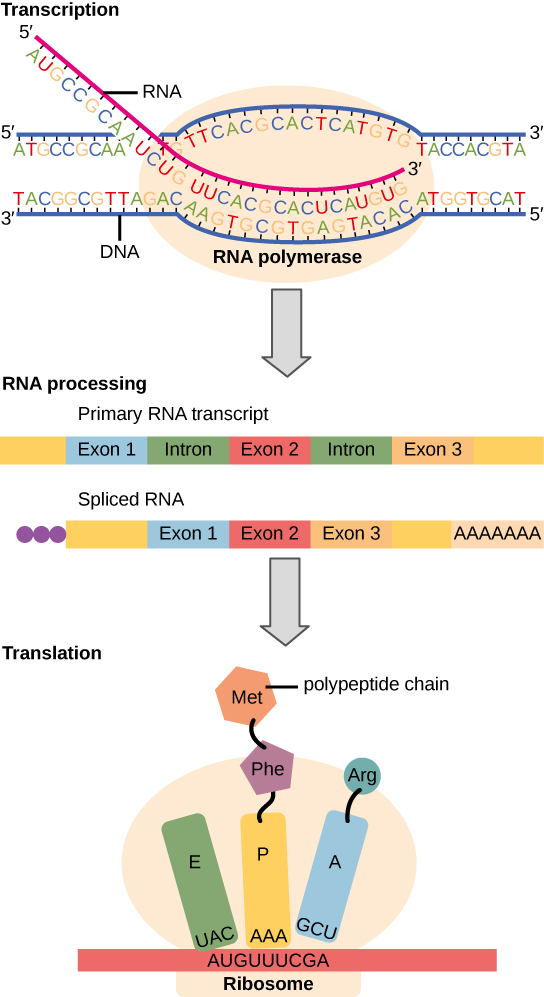
\includegraphics[width=0.6\linewidth]{./../images/central_dogma_genetics} \caption{The central dogma of biology}\label{fig:central-dogma}
\end{figure}

\ecolumns
\end{frame}

\begin{frame}{Terminologies}
\protect\hypertarget{terminologies}{}
\begin{table}

\caption{\label{tab:gene-terms1}Some terms applicable in the context of genetic code}
\centering
\fontsize{6}{8}\selectfont
\begin{tabular}[t]{>{\raggedright\arraybackslash}p{8em}>{\raggedright\arraybackslash}p{38em}}
\toprule
Term & Meaning\\
\midrule
\textbf{\cellcolor{gray!6}{Code letter}} & \cellcolor{gray!6}{A nucleotide e.g., A, U, G, C (in mRNA) or A, T, G, C (in DNA)}\\
\textbf{Code word} & A sequence of nucleotides specifying an amino acid. e.g., the RNA codon for leucine = CUG (of GAC for DNA)\\
\textbf{\cellcolor{gray!6}{Anticodon}} & \cellcolor{gray!6}{A sequence of nucleotides on tRNA that complements the codon, e.g., GAC = anticodon for leucine}\\
\textbf{Word size of codon} & The number of letters in a code word, e.g., three letters in a triplet code. These are the same as coding ratio in a nonoverlapping code.\\
\textbf{\cellcolor{gray!6}{Non overlapping code}} & \cellcolor{gray!6}{A code in which only as many amino acids are coded as there are code words in end-to-end sequence, e.g., for a triplet code UUUCCC = phenylalanine (UUU) + proline (CCC)}\\
\addlinespace
\textbf{Overlapping code} & When more amino acids are coded for in a single reading frame than there are code words present in end-to-end sequence, e.g., UUUCCC = phenylalanine (UUU) + phenylalanine (UUU) + serine (UCC) + proline (CCC)\\
\textbf{\cellcolor{gray!6}{Nondegenerate code}} & \cellcolor{gray!6}{When there is only one codon for each amono acid, e.g., 20 different amino acids have a total of 20 codons.}\\
\textbf{Degenerate code} & When there is more than one codon for a particular amino acid, e.g., UUU, UUC = phenylalanine, or 20 different amino acids have a total of more than 20 codons.\\
\bottomrule
\end{tabular}
\end{table}
\end{frame}

\begin{frame}{}
\protect\hypertarget{section-2}{}
\begin{table}

\caption{\label{tab:gene-terms2}Some terms applicable in the context of genetic code (...continued)}
\centering
\fontsize{6}{8}\selectfont
\begin{tabular}[t]{>{\raggedright\arraybackslash}p{8em}>{\raggedright\arraybackslash}p{40em}}
\toprule
Term & Meaning\\
\midrule
\textbf{\cellcolor{gray!6}{Synonymous codons}} & \cellcolor{gray!6}{Different codons that specify the same amino acid in a degenerate code, e.g., UUU = UUC = phenylalanine}\\
\textbf{Ambigious code} & When one codon can code for more than one amino acid, e.g., GGA = glycine, glutamic acid\\
\textbf{\cellcolor{gray!6}{Commaless code}} & \cellcolor{gray!6}{When there are no intermediary nucleotides (spacers) between words, e.g., UUUCCC = two amino acids in triplet nonoverlapping code}\\
\textbf{Reading frame} & The particular nucleotide sequence, coding for a polypeptide, that starts at a specific point and is then partitioned into codon until the final code word of that sequence is reached.\\
\textbf{\cellcolor{gray!6}{Frameshift mutation}} & \cellcolor{gray!6}{A change in the reading frame because of the insertion or deletion of nucleotides in numbers other than multiples of the codon length. This modifies the previous partitioning of codons in the reading frame, and causes a new sequence of codons to be read.}\\
\addlinespace
\textbf{Sense word} & A codon that specifies an amino acid normally present at that position in a protein\\
\textbf{\cellcolor{gray!6}{Missense mutation}} & \cellcolor{gray!6}{A change in nucleotide sequence, either by deletion, insertion, or subsitution, resulting in the appearance of a codon that produces a different amino acid in a particular protein, e.g., UUU (phenylalanine) mutates to UGU (Cysteine)}\\
\textbf{Nonsense mutation} & A mutation that results in a codon that does not produce an amino acid, e.g., UAG (also called a “stop” mutation or “chain termination” codon)\\
\textbf{\cellcolor{gray!6}{Universality}} & \cellcolor{gray!6}{Utilization of the same genetic code in all organisms, e.g. UUU = phenylalanine in bacteria, mouse, man and tobacco (with some exceptions in mitochondria)}\\
\bottomrule
\end{tabular}
\end{table}
\end{frame}

\begin{frame}{Genetic code: The search}
\protect\hypertarget{genetic-code-the-search}{}
\begin{itemize}
\tightlist
\item
  Evidence first presented on its nature in 1961 by Francis Crick and
  Sydney Brenner used the chemical mutagen proflavin to insert (+) or
  delete (-) one, two, or three nucleotides into the gene of a virus.

  \begin{itemize}
  \tightlist
  \item
    When one or two nucleotides were inserted/deleted, protein synthesis
    was completely abolished. When three nucleotides were
    inserted/deleted, the protein was synthesized and functional.
  \item
    The insertion/deletion of one or two nucleotides completely changed
    the triplet reading frame, thereby altering the message for every
    subsequent amino acid.
  \item
    Insertion/deletion of three nucleotides caused an extra amino acid
    to be inserted during translation, the integrity of the rest of the
    protein was maintained.
  \end{itemize}
\end{itemize}
\end{frame}

\begin{frame}{Nature: Code triplet}
\protect\hypertarget{nature-code-triplet}{}
\begin{itemize}
\tightlist
\item
  Given the different numbers of ``letters'' in the mRNA and protein
  ``alphabets,'' scientists theorized that combinations of nucleotides
  corresponded to single amino acids.
\item
  These nucleotide triplets are called
  codons\footnote[frame]{Codons: Three consecutive nucleotides in mRNA that specify the insertion of an amino acid or the release of a polypeptide chain during translation}.
\item
  Nucleotide doublets would not be sufficient to specify every amino
  acid because there are only 16 possible two-nucleotide combinations.
\end{itemize}

\begin{align}
\begin{split}
4^2 &= 16 \nonumber \\
4^3 &= 64
\end{split}
\end{align}

\begin{itemize}
\tightlist
\item
  If there were 200 commonly occurring amino acids instead of 20. Given
  what you know about the genetic code, what would be the shortest
  possible codon length? Explain.
\end{itemize}
\end{frame}

\begin{frame}{Nature: Degeneracy}
\protect\hypertarget{nature-degeneracy}{}
\begin{itemize}
\tightlist
\item
  Scientists theorized that amino acids were encoded by nucleotide
  triplets and that the genetic code was
  degenerate\footnote[frame]{(of the genetic code) describes that a given amino acid can be encoded by more than one nucleotide triplet}.
\item
  Scientists solved the genetic code by translating synthetic mRNAs in
  vitro and sequencing the proteins they specified
\item
  In addition to instructing the addition of a specific amino acid to a
  polypeptide chain, three of the 64 codons terminate protein synthesis
  and release the polypeptide from the translation machinery. These
  triplets are called nonsense
  codons\footnote[frame]{one of the three mRNA codons that specifies termination of translation},
  or stop codons.
\item
  AUG codon has a special function.

  \begin{itemize}
  \tightlist
  \item
    Specifies the amino acid methionine,
  \item
    Serves as the start codon to initiate translation. The reading frame
    for translation is set near the 5' end of the mRNA.
  \end{itemize}
\end{itemize}
\end{frame}

\begin{frame}{Nature: Universality}
\protect\hypertarget{nature-universality}{}
\begin{itemize}
\tightlist
\item
  The genetic code is universal. With a few exceptions, virtually all
  species use the same genetic code for protein synthesis.
\item
  Conservation of codons means that a purified mRNA encoding the globin
  protein in horses could be transferred to a tulip cell, and the tulip
  would synthesize horse globin.
\item
  That there is only one genetic code is powerful evidence that all of
  life on Earth shares a common origin, especially considering that
  there are about \(10^{84}\) possible combinations of 20 amino acids
  and 64 triplet codons.
\end{itemize}
\end{frame}

\begin{frame}{}
\protect\hypertarget{section-3}{}
\begin{figure}
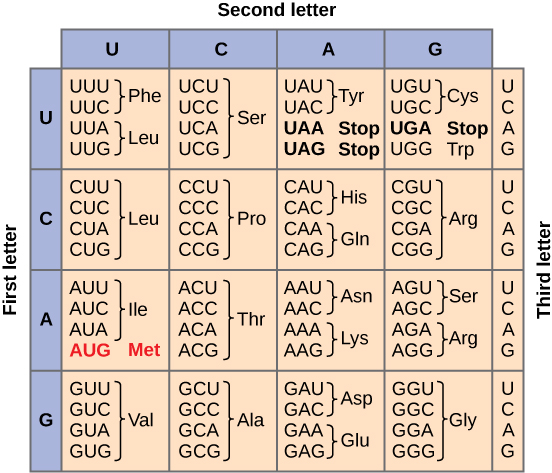
\includegraphics[width=0.45\linewidth]{./../images/nucleotide_codons} \caption{The genetic code is universal for all life forms}\label{fig:universality}
\end{figure}
\end{frame}

\begin{frame}{Property: Overlapping/non-overlapping genetic code}
\protect\hypertarget{property-overlappingnon-overlapping-genetic-code}{}
\begin{figure}
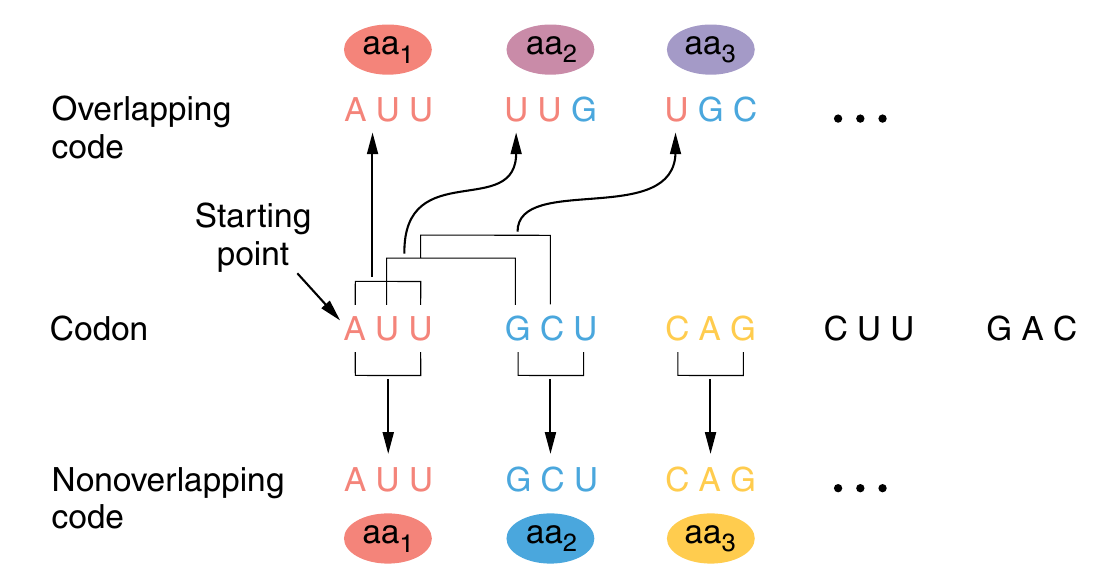
\includegraphics[width=0.4\linewidth]{./../images/overlap_non_overlap} \caption{Overlapping versus non overlapping genetic codes}\label{fig:overlap-n-non}
\end{figure}

\begin{itemize}
\tightlist
\item
  An overlapping and a nonoverlapping genetic code would translate
  differently into an amino acidc sequence.
\item
  In an overlapping code, single nucleotides occupy positions in
  multiple codons.
\item
  In a nonoverlapping code, a protein is translated by reading
  nucleotides sequentially in sets of three.
\end{itemize}
\end{frame}

\begin{frame}{Property}
\protect\hypertarget{property}{}
\begin{itemize}
\tightlist
\item
  With comma/commaless
\item
  Non-ambiguous
\end{itemize}
\end{frame}

\begin{frame}{Translational consequences of a mutation}
\protect\hypertarget{translational-consequences-of-a-mutation}{}
\begin{figure}
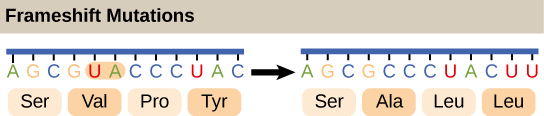
\includegraphics[width=0.45\linewidth]{./../images/frameshift_mutation} \caption{Frameshift mutation}\label{fig:frameshift-mutation}
\end{figure}

\begin{itemize}
\tightlist
\item
  Degeneracy is believed to be a cellular mechanism to reduce the
  negative impact of random mutations.
\item
  Codons that specify the same amino acid typically only differ by one
  nucleotide.
\item
  Amino acids with chemically similar side chains are encoded by similar
  codons.
\item
  So what does single nucleotide mutation do ?
\end{itemize}
\end{frame}

\begin{frame}{Molecular phenotype}
\protect\hypertarget{molecular-phenotype}{}
\begin{itemize}
\tightlist
\item
  The primary phenotype of a gene is the protein it produces.
\item
  Two variants of a gene -- wild and mutant, produce functionally
  different proteins to be called alleles.
\item
  Human disease phenylketonuria (PKU) provides a hint to the topic.
\end{itemize}
\end{frame}

\begin{frame}{Molecular biology of PKU}
\protect\hypertarget{molecular-biology-of-pku}{}
\begin{itemize}
\tightlist
\item
  Due to defective allele of a gene that encodes for liver enzyme
  phenylalanine hydroxylase (PAH).
\end{itemize}

\[
\begin{aligned}
\textrm{phenylalanine} \xrightarrow{\text{phenylalanine hydroxylase}} \textrm{tyrosine}
\end{aligned}
\]

\begin{itemize}
\tightlist
\item
  A mutation in the gene encoding this enzyme may alter the amino acid
  sequence in the vicinity of the enzyme's active site. In this case,
  the enzyme cannot bind phenylalanine or convert it into tyrosine.
\item
  Phenylalanine builds up and is instead converted into phenylpyruvic
  acid, this interferes with the development of the nervous system.
\end{itemize}
\end{frame}

\begin{frame}{}
\protect\hypertarget{section-4}{}
\begin{itemize}
\tightlist
\item
  Mutations occur at different sites along the gene. Functional
  mutations are essentially those occurring in the protein-encoding
  regions, or the exons. They represent a range of DNA changes, but most
  are small changes affecting only one nucleotide pair among the
  thousands that constitute the gene.
\item
  By changing one or more amino acids, (non-synonymous) mutations
  inactivate some essential part of the protein encoded by the gene. The
  effect of the mutation on the function of the gene depends on where
  within the gene the mutation occurs.
\end{itemize}
\end{frame}

\begin{frame}{}
\protect\hypertarget{section-5}{}
\begin{itemize}
\tightlist
\item
  An important functional region of the gene is that encoding an
  enzyme's active site. In addition, a minority of mutations are found
  to be in introns, and these mutations often prevent the normal
  processing of the primary RNA transcript.
\item
  Many of the mutant alleles are of a type generally called null
  alleles: the proteins encoded by them completely lack PAH function.
  Other mutant alleles reduce the level of enzyme function; they are
  sometimes called leaky mutations, because some wild-type function
  seems to ``leak'' into the mutant phenotype.
\end{itemize}
\end{frame}

\hypertarget{one-gene-one-polypeptide-hypothesis}{%
\section{One gene one polypeptide
hypothesis}\label{one-gene-one-polypeptide-hypothesis}}

\begin{frame}{Functionality of genes}
\protect\hypertarget{functionality-of-genes}{}
\begin{itemize}
\tightlist
\item
  Genes don't always encode protein
\item
  Some genes encode RNAs that have special functions, however all genes
  are transcribed to make RNA.
\item
  RNAs that do not end up being mRNAs are functional RNAs (ribosomal
  RNAs, small cytoplasmic RNAs).
\end{itemize}
\end{frame}

\begin{frame}{Study in \emph{Neurospora} fungus}
\protect\hypertarget{study-in-neurospora-fungus}{}
\begin{itemize}
\tightlist
\item
  Genes act by controlling cellular chemistry.
\item
  Beadle and Tatum received a Nobel Prize for their study on the haploid
  fungus \emph{Neurospora}.
\item
  They used forward genetic approach by first inducing mutations and
  then tested cultures grown from ascospores for interesting mutant
  phenotypes.
\item
  Specifially auxotrophic mutants were the subject; Auxotrophic mutants
  cannot synthesize all its cellular components from the inorganic
  nutrients and a carbon source in the medium.
\item
  Thus mutant is defective for some normal synthesyzing step.
\end{itemize}
\end{frame}

\begin{frame}{}
\protect\hypertarget{section-6}{}
\begin{itemize}
\tightlist
\item
  It was first confirmed that each mutation that generated a nutrient
  requirement was inherited as a single-gene mutation because each gave
  a 1:1 ratio when crossed with a wild type. Letting \emph{aux}
  represent auxotrophic mutation and wild type as ``+'',
\end{itemize}

\[
\begin{aligned}
+ &\times aux \\
 &\downarrow\\
\textrm{progeny}: \frac{1}{2} + &\textrm{and} \frac{1}{2}aux
\end{aligned}
\]

\begin{itemize}
\tightlist
\item
  The second step was to classify the specific nutritional requirement
  of each auxotroph.
\item
  Some grew only if proline was supplied, others methionine, others
  pyridoxine, others arginine. Focus was set on arginine types.
\item
  Three separate genes different loci were identified on separate
  chromosomes.
\item
  It was discovered that auxotrophs for each of the three loci differed
  in their response to the structurally related compounds ornithine and
  citrulline.
\end{itemize}
\end{frame}

\begin{frame}{}
\protect\hypertarget{section-7}{}
\begin{itemize}
\tightlist
\item
  \emph{arg-1} mutants grew when supplied with any one of the chemicals
  ornithine, citrulline, or arginine.
\item
  \emph{arg-2} mutants grew when either citrulline or arginine was
  supplied.
\item
  \emph{arg-3} mutants grew only when arginine was supplied.
\item
  Enzymes were already known to interconvert such related compounds.
\item
  B \& P proposed a biochemical pathway for such conversion in the
  fungus:
\end{itemize}

\[
\begin{aligned}
\textrm{precursor} \xrightarrow{\text{enzyme X}} \textrm{ornithine} \xrightarrow{\text{enzyme Y}} \textrm{citrulline} \xrightarrow{\text{enzyme Z}} \textrm{arginine}
\end{aligned}
\]

\begin{figure}
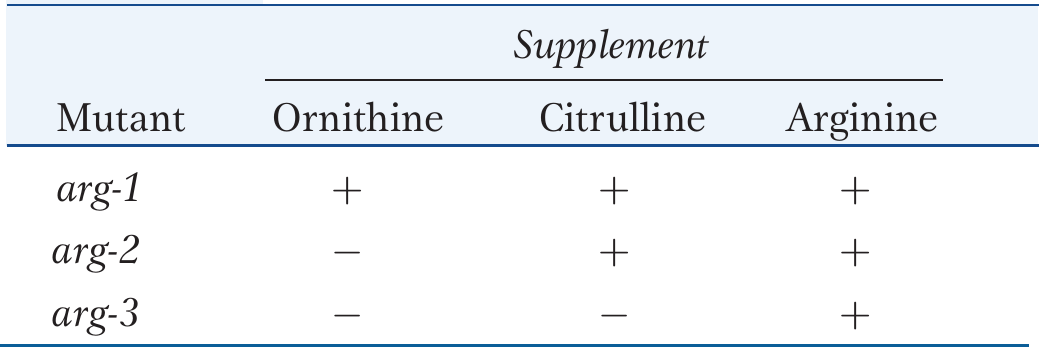
\includegraphics[width=0.4\linewidth]{./../images/mutant_growth_supplements} \caption{Growth of \textit{arg} Mutants in response to supplements.}\label{fig:mutants-supplements}
\end{figure}
\end{frame}

\begin{frame}{}
\protect\hypertarget{section-8}{}
\begin{itemize}
\tightlist
\item
  The model:

  \begin{itemize}
  \tightlist
  \item
    \emph{arg-1} mutants have a defective enzyme X, and so they are
    unable to convert the precursor into ornithine as the first step in
    producing arginine. However they have normal enzymes Y and Z, and so
    the arg-1 mutants are able to produce arginine if supplied with
    either ornithine or citrulline.
  \item
    \emph{arg-2} mutants lack enzyme Y, and the \emph{arg-3} mutants
    lack enzyme Z.
  \item
    A mutation at a particular gene is assumed to interfere with the
    production of a single enzyme.
  \item
    The defective enzyme creates a block in biosynthetic pathway. The
    block can be prevented by supplying to the cells any compound that
    normally comes after the block in the pathway.
  \end{itemize}
\end{itemize}

\[
 \text{Precursor} \xrightarrow 
 {
 \begin{subarray}{c}
 arg-1^+ \\
 \downarrow \\
 \text{Enzyme X}
 \end{subarray}
 } 
 \text{Ornithine} \xrightarrow
  {
 \begin{subarray}{c}
  arg-2^+ \\
 \downarrow \\
 \text{Enzyme Y}
 \end{subarray}
 }
 \text{Citrulline} \xrightarrow
  {
 \begin{subarray}{c}
  arg-3^+ \\
 \downarrow \\
 \text{Enzyme Z}
 \end{subarray}
 }
 \text{Arginine}
\]
\end{frame}

\begin{frame}{}
\protect\hypertarget{section-9}{}
\begin{itemize}
\tightlist
\item
  This model was initially known as the \emph{one-gene-one-enzyme
  hypothesis}.
\item
  Genes somehow were responsible for the function of enzymes, and each
  gene appar- ently controlled one specific enzyme in a series of
  interconnected steps in a bio- chemical pathway
\item
  All \textbf{Proteins} are infact encoded by gene hence the phrase
  one-gene-one-polypeptide hypothesis.
\item
  Hence Beadle and Tatum's hypothesis became the great unifying theory
  that brought together areas of genetics and biochemistry together.
\end{itemize}
\end{frame}

\hypertarget{enzymatic-explanation-of-genetic-ratios}{%
\section{Enzymatic explanation of genetic
ratios}\label{enzymatic-explanation-of-genetic-ratios}}

\begin{frame}{}
\protect\hypertarget{section-10}{}
\begin{itemize}
\tightlist
\item
  An enzyme is a product of gene/s.

  \begin{itemize}
  \tightlist
  \item
    A tertiary or quarternary form of polypeptide derived from
    amino-acid units.
  \end{itemize}
\item
  Enzyme controls/catalyzes biochemical reaction and the reaction
  produces biochemical product which is responsible to final phenotype
  expression.
\item
  So, phenotypic ratio is determined by the enzyme.
\end{itemize}
\end{frame}

\begin{frame}{The 9:3:3:1 ratio; No interaction}
\protect\hypertarget{the-9331-ratio-no-interaction}{}
\begin{itemize}
\tightlist
\item
  In inheritance of skin coloration in corn snakes, the phenotype is
  produced by two separate pigments. The snake's natural color is a
  repeating black and orange camouflage pattern, as shown in Figure
  \ref{fig:gene-no-interaction1} (a).
\item
  The phenotype is produced by two separate pigments, both of which are
  under genetic control.
\item
  One gene determines orange pigment (\(o^+\) and \(o\)) and another
  gene determines black pigment (\(b^+\) and \(b\)).
\item
  Two genes are unlinked.
\item
  Natural pattern is produced by the genotype \(o^+/\_;\ b+/\_\).
\item
  What genotypes leads to completely black pigmentation?
\end{itemize}
\end{frame}

\begin{frame}{}
\protect\hypertarget{section-11}{}
\begin{figure}

{\centering 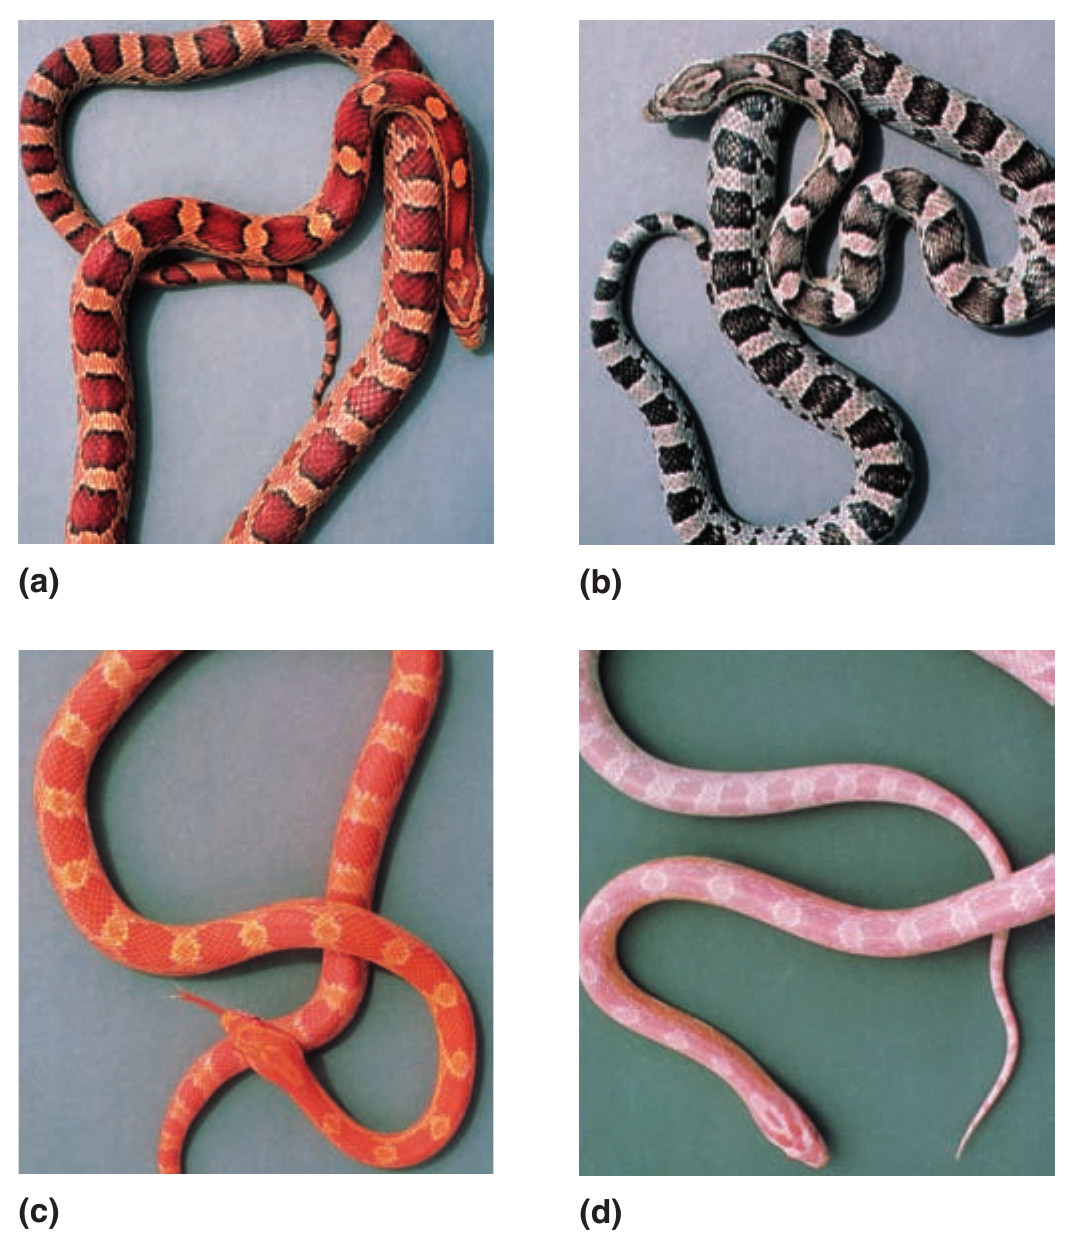
\includegraphics[width=0.42\linewidth]{./../images/gene_no_interaction} 

}

\caption{Phenotypes of snake skin pigmentation}\label{fig:gene-no-interaction1}
\end{figure}
\end{frame}

\begin{frame}{}
\protect\hypertarget{section-12}{}
\begin{itemize}
\tightlist
\item
  If homozygous orange and a homozygous black snake are crossed, the
  \(F_1\) is wild type (camouflaged), demonstrating complementation.
\end{itemize}

\begin{center}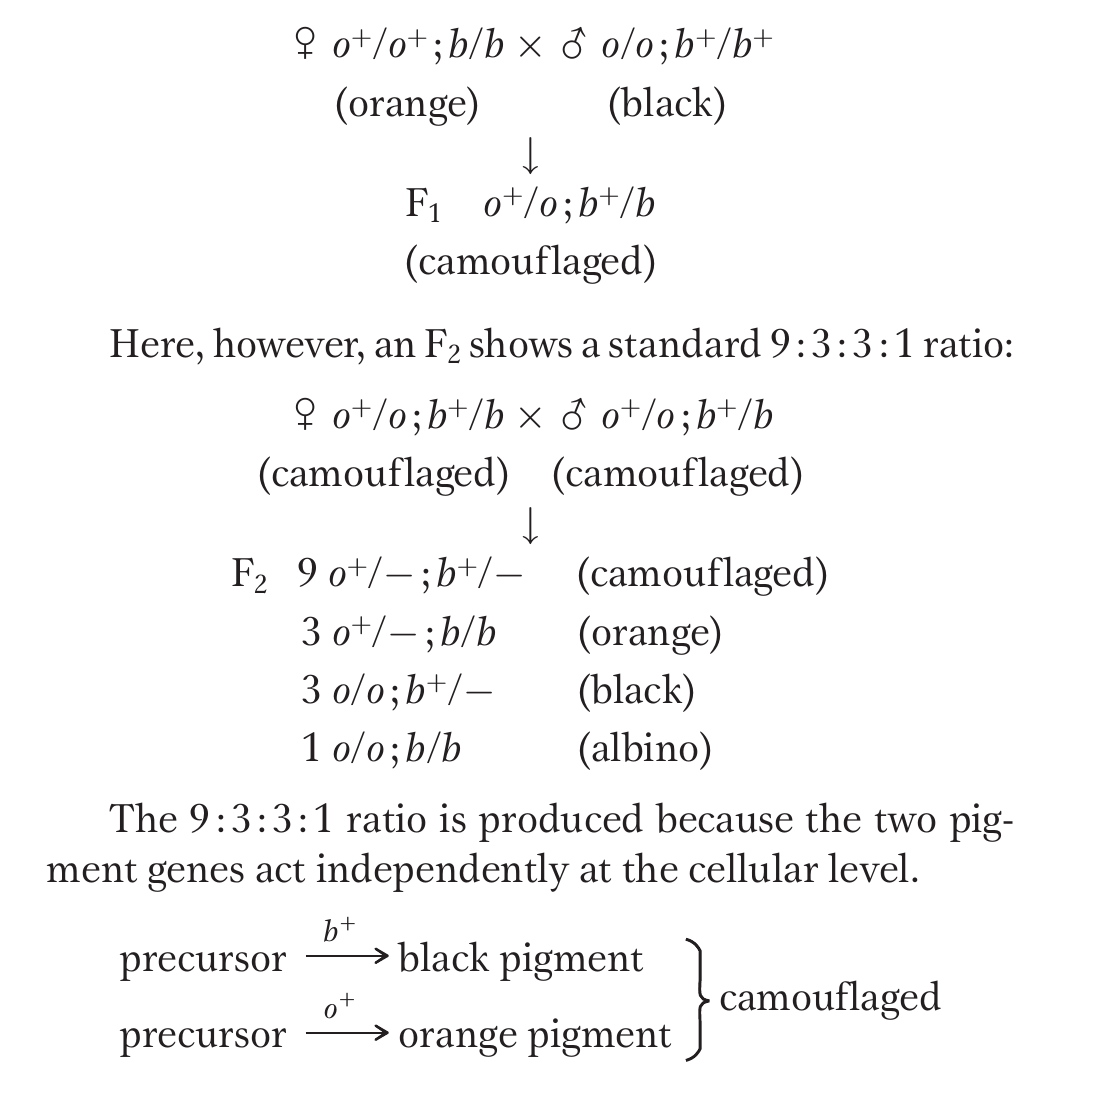
\includegraphics[width=0.4\linewidth]{./../images/gene_no_interaction2} \end{center}
\end{frame}

\begin{frame}{The 9:7 ratio: gene complementation (genes acting on same
pathway)}
\protect\hypertarget{the-97-ratio-gene-complementation-genes-acting-on-same-pathway}{}
\begin{itemize}
\tightlist
\item
  The \(F_2\) ratio from the harbell dihybrid cross shows both blue and
  white plants in ratio of 9:7. How can such results be explained ?
\item
  The 9:7 ratio is a modification of the dihybrid 9:3:3:1 ratio with the
  3:3:1 combined to make 7.
\end{itemize}
\end{frame}

\begin{frame}{}
\protect\hypertarget{section-13}{}
\begin{columns}[T,onlytextwidth]
  \footnotesize
  \column{0.5\textwidth}
  

\begin{center}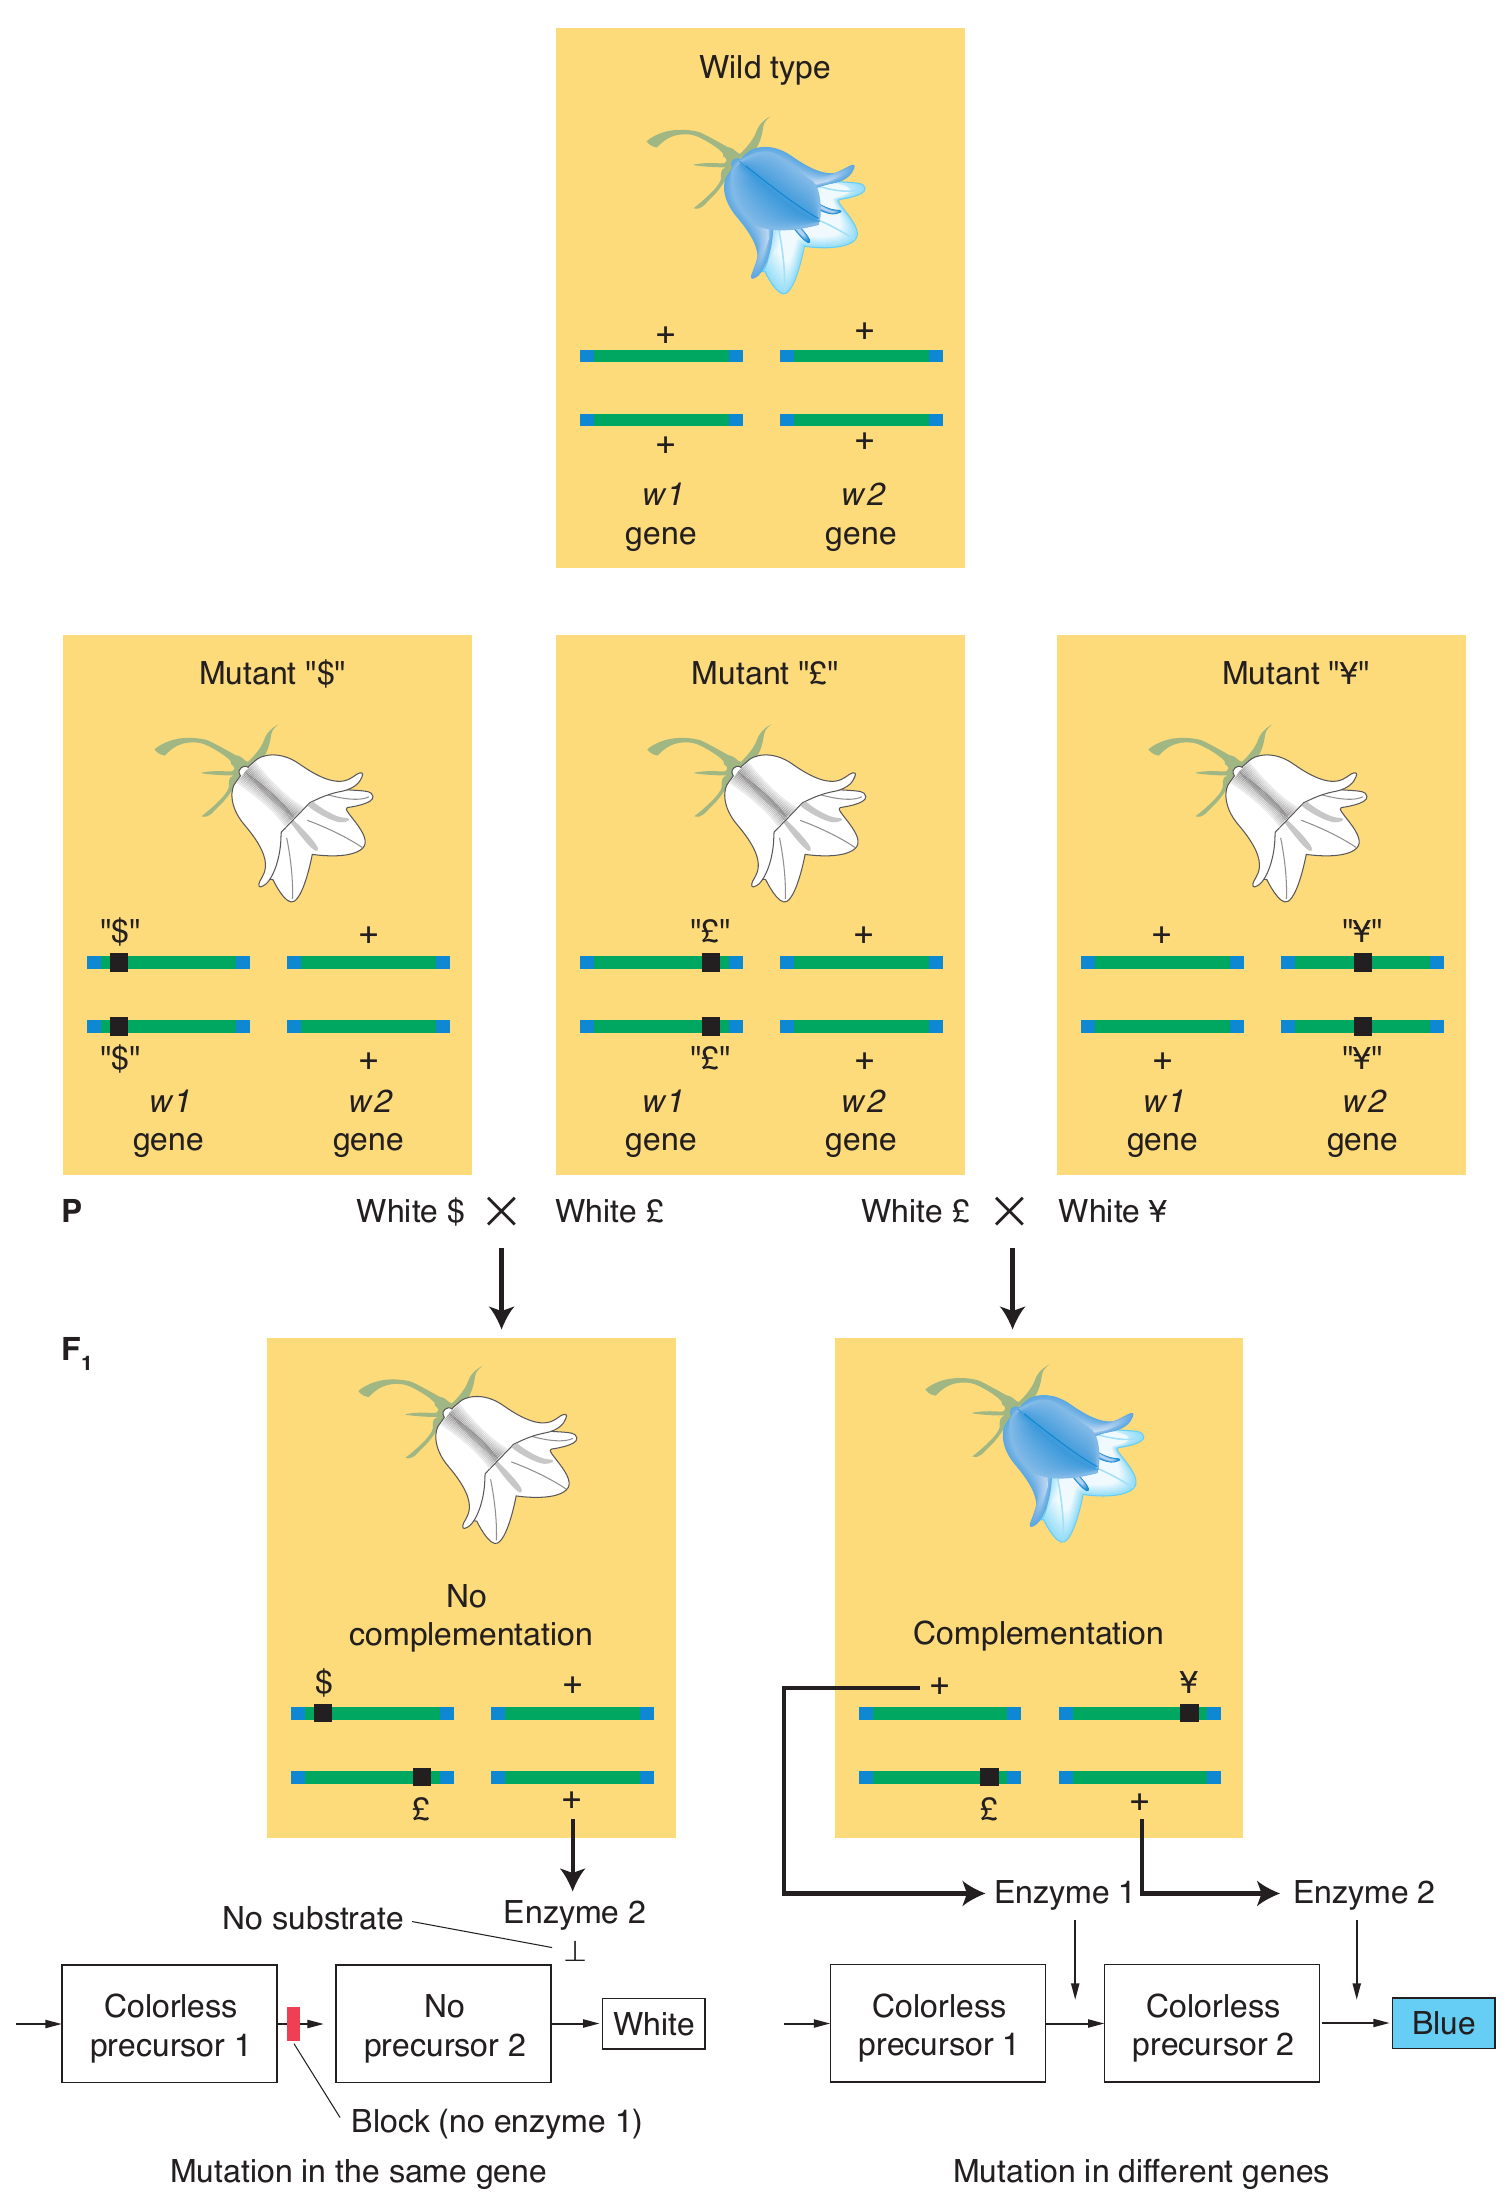
\includegraphics[width=0.68\linewidth]{./../images/gene_complementation} \end{center}

  \column{0.5\textwidth}


\begin{center}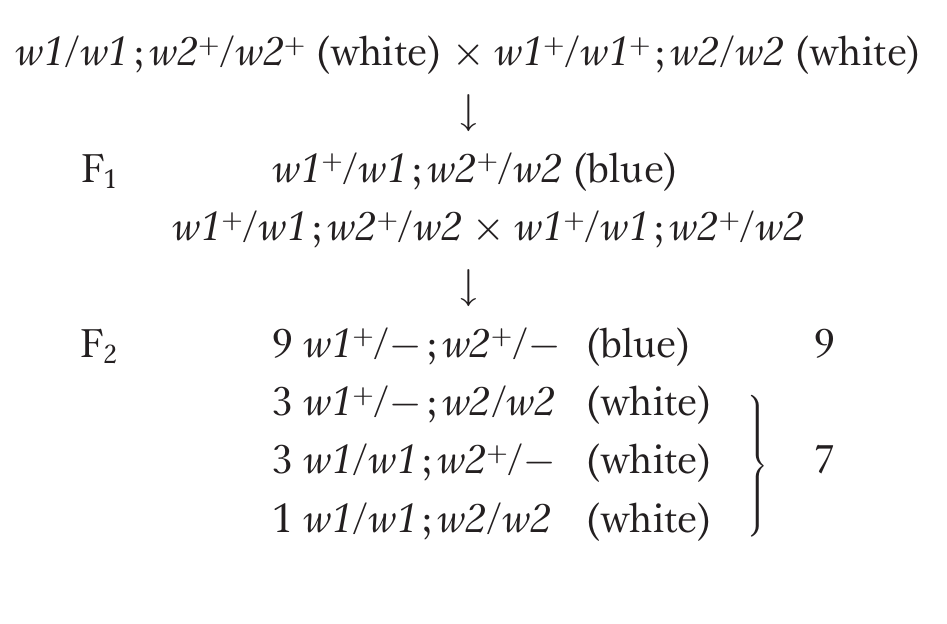
\includegraphics[width=0.8\linewidth]{./../images/gene_same_pathway} \end{center}
  
\end{columns}
\end{frame}

\begin{frame}{}
\protect\hypertarget{section-14}{}
\begin{itemize}
\tightlist
\item
  Only way in which a 9:7 ratio is possible is if the double mutant has
  the same phenotypes as the two single mutants.
\item
  Hence, the modified ratio constitutes a way of identifying the double
  mutant's phenotype.
\item
  Furthermore, the identical phenotypes of the single and double mutants
  suggest that each mutant allele controls a different step in the same
  pathway.
\item
  The results show that a plant will have white petals if it is
  homozygous for the recessive mutant allele of either gene or both
  genes.
\item
  To have the blue phenotype, a plant must have at least one copy of the
  dominant allele of both genes because both are needed to complete the
  sequential steps in the pathway.
\item
  No matter which is absent, the same pathway fails, producing the same
  phenotype. The enzymatic pathways allowing for complementation is
  through regulatory gene products (Shown in
  \ref{fig:functional-regulatory-gene}).
\item
  Thus, three of the genotypic classes will produce the same phenotype,
  and so, overall, only two phenotypes result.
\end{itemize}
\end{frame}

\begin{frame}{The 9:3:4 ratio: recessive epistasis}
\protect\hypertarget{the-934-ratio-recessive-epistasis}{}
\begin{itemize}
\tightlist
\item
  One important type of functional interaction between different genes
  occurs when an allele of genotype at one locus ``masks'' or inhibits
  the expression of a allele or genotype at a different locus, such an
  interaction is called epistasis.
\item
  Epistasis means stand upon.
\item
  Double mutants show the phenotype of one mutation but not the other.
\item
  Overriding mutation is epistatic, whereas the overridden one is
  hypostatic.
\item
  Also results from the genes in same pathway.
\item
  In a simple model, if epistatic mutation is carried by a gene that if
  farther upstream than the one being overridden, the mutant phenotype
  of the upstream gene takes precedence, no matter what is taking place
  later in the pathway.
\end{itemize}
\end{frame}

\begin{frame}{}
\protect\hypertarget{section-15}{}
\[
\begin{aligned}
& & w/w; m^+/m^+ (\text{white}) & \times w^+/w^+; m/m (\text{magenta}) &\\
& \mathrm{F_1} & & w^+/w; m^+/m (\text{blue}) & \\
& & & \downarrow & \\
& & w^+/w; m^+/m &\times w^+/w; m^+/m & \\
& & & \downarrow & \\
& \mathrm{F_2} & & 9w^+/\_; m^+/\_ (\text{blue}) \hspace{1cm} & 9 \\
& & & 3 w^+/\_; m/m (\text{magenta}) \hspace{1cm} & 3 \\
& & & \left\{
\begin{array}{ll}
3 w/w; m^+/\_ (\text{white}) \hspace{1cm} \\
1 w/w; m/m (\text{white})
\end{array}
\right\} & 4
\end{aligned}
\]
\end{frame}

\begin{frame}{}
\protect\hypertarget{section-16}{}
\begin{figure}

{\centering 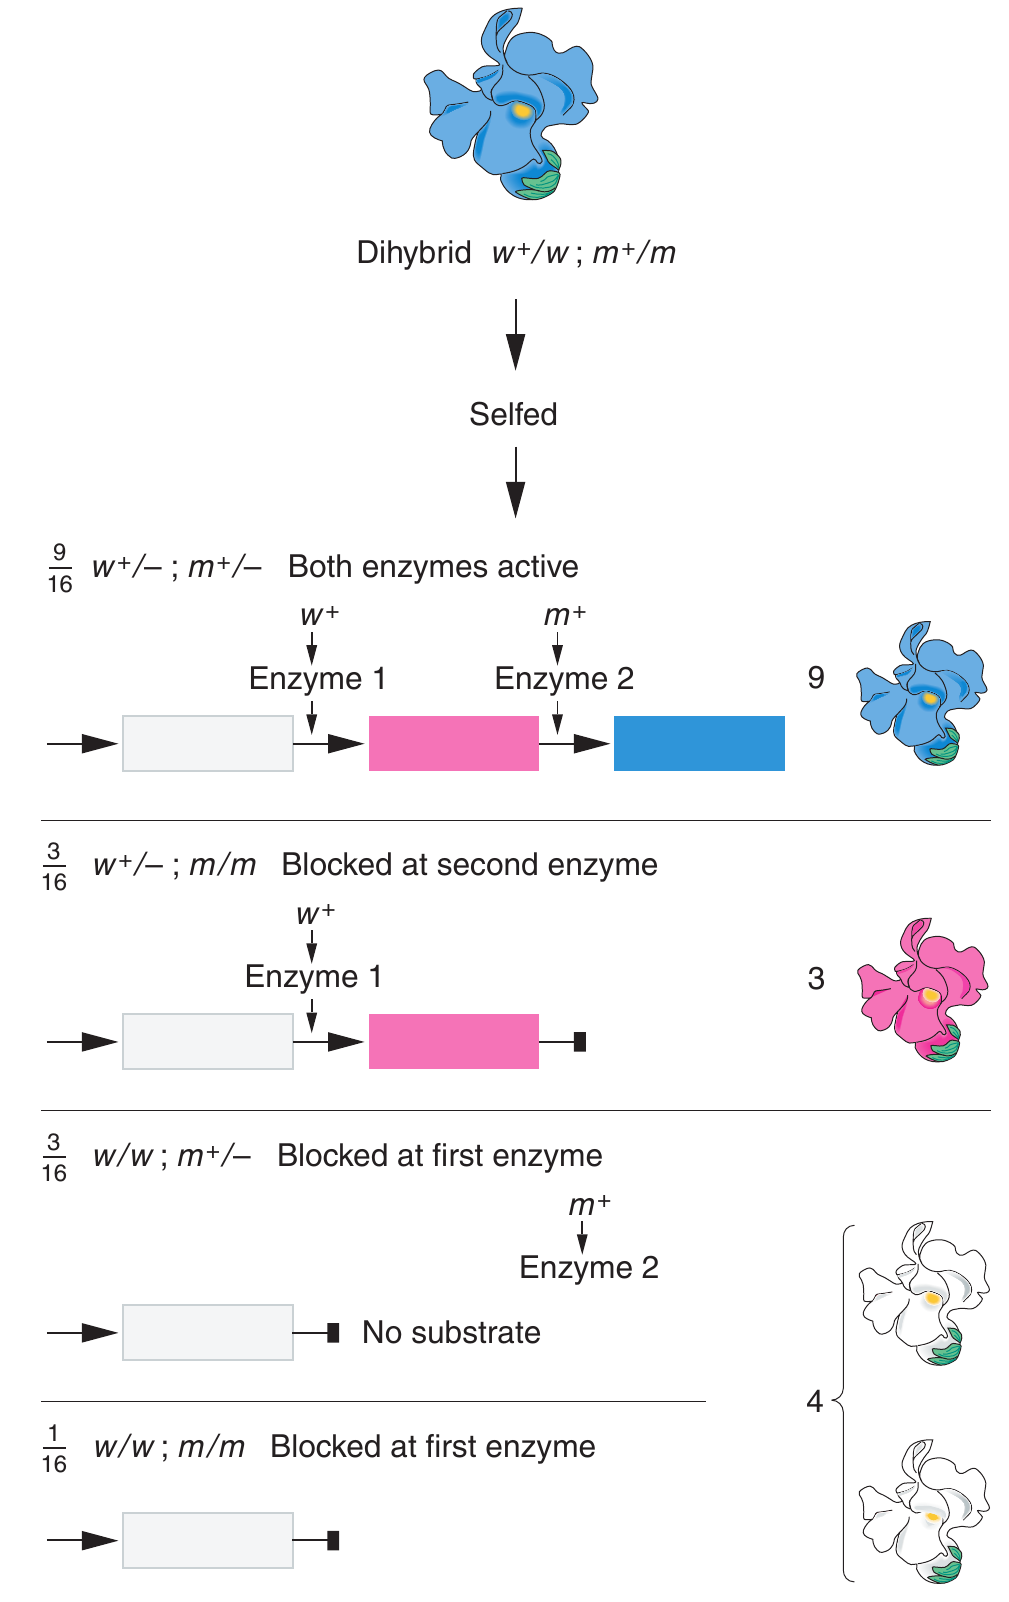
\includegraphics[width=0.3\linewidth]{./../images/recessive_epistasis} 

}

\caption{A model for recessive epistasis}\label{fig:recessive-epistasis}
\end{figure}
\end{frame}

\begin{frame}{}
\protect\hypertarget{section-17}{}
\begin{block}{}
Epistasis is inferred when a mutant allele of one gene masks the expression of a mutant allele of another gene and expresses its own phenotype instead.
\end{block}

\begin{itemize}
\tightlist
\item
  This interaction is called recessive epistasis because a recessive
  phenotype (white) overrides the other phenotype.
\item
  At the cellular level, we can account for the recessive epistasis in
  \emph{Collinsia} by the following type of pathway.
\end{itemize}

\[
\begin{aligned}
\textrm{colorless} \xrightarrow{\text{gene}~w^+} \textrm{magenta} \xrightarrow{\text{gene}~m^+} \textrm{blue}
\end{aligned}
\]

\begin{itemize}
\tightlist
\item
  Notice that the epistatic mutation occurs in a step in the pathway
  leading to blue pigment; this step is upstream of the step that is
  blocked by the masked mutation.
\end{itemize}
\end{frame}

\begin{frame}{The 12:3:1 ratio: dominant epistasis}
\protect\hypertarget{the-1231-ratio-dominant-epistasis}{}
\begin{itemize}
\tightlist
\item
  In foxgloves ( \emph{Digitalis purpurea}), two genes interact in the
  pathway that determines petal coloration.
\item
  The two genes are unlinked.
\item
  One gene affects the intensity of red pigment in the petal,

  \begin{itemize}
  \tightlist
  \item
    \emph{d} results in the light red color seen in natural populations
  \item
    \emph{D} is a mutant allele that produces dark red color.
  \end{itemize}
\item
  Other gene determines in which cells the pigment is synthesized,

  \begin{itemize}
  \tightlist
  \item
    \emph{w} allows synthesis of the pigment throughout the petals as in
    the wild type,
  \item
    \emph{W} is a mutant allele that confines pigment synthesis to the
    small throat spots.
  \end{itemize}
\item
  Selfing of dihybrid shows:
\end{itemize}
\end{frame}

\begin{frame}{}
\protect\hypertarget{section-18}{}
\[
\begin{aligned}
& \left\{
\begin{array}{ll}
9D/\_; W/\_ (\textrm{white with spots}) \hspace{1cm} \\
3 d/d; W/\_ (\textrm{white with spots}) \hspace{1cm}
\end{array}
\right\} & 12 \\
& 3 D/\_; w/w (\textrm{dark with red}) \hspace{1cm} & 3 \\
& 1 d/d; w/w (\textrm{light red}) & 1
\end{aligned}
\]
\end{frame}

\begin{frame}{}
\protect\hypertarget{section-19}{}
\begin{figure}

{\centering 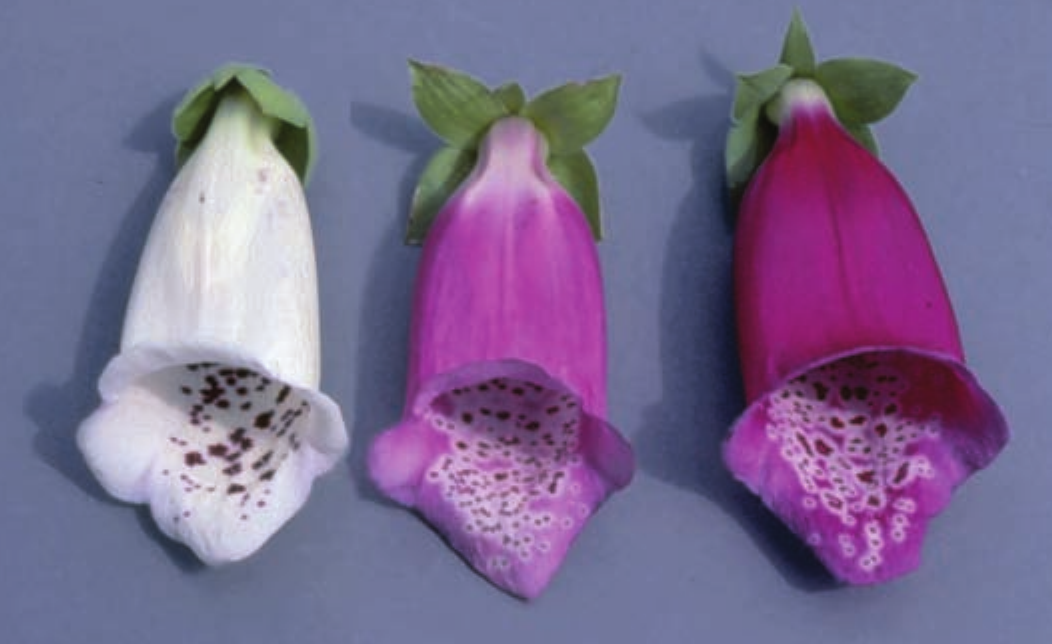
\includegraphics[width=0.4\linewidth]{./../images/dominant_epistasis} 

}

\caption{Dominant epistasis due to white mutation}\label{fig:dominant-epistasis}
\end{figure}
\end{frame}

\begin{frame}{Regulators}
\protect\hypertarget{regulators}{}
\begin{figure}

{\centering 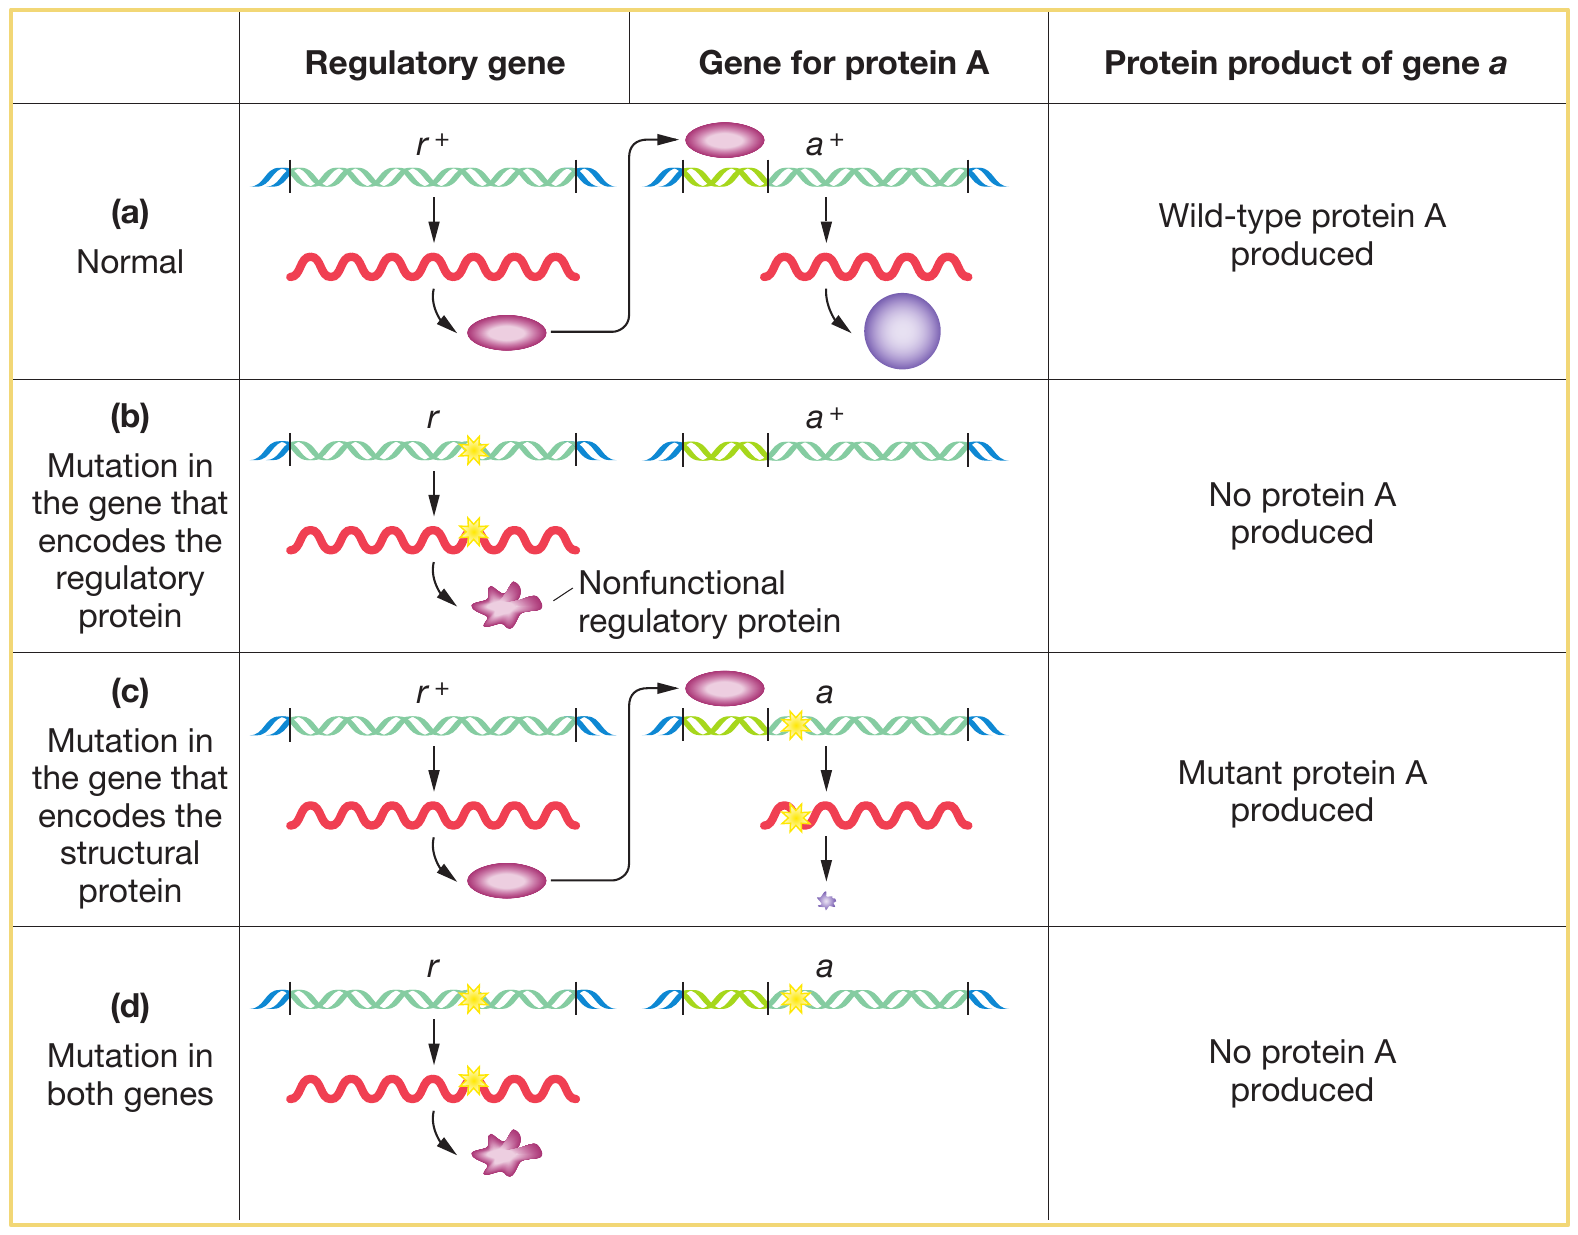
\includegraphics[width=0.48\linewidth]{./../images/genes_in_same_pathway_biochemical} 

}

\caption{\textbf{Molecular mechanisms of genes acting on same pathway.} Interaction between a regulatory protein and its target}\label{fig:functional-regulatory-gene}
\end{figure}
\end{frame}

\begin{frame}{Suppressors}
\protect\hypertarget{suppressors}{}
\begin{itemize}
\tightlist
\item
  A suppressor is a mutant allele of a gene that reverses the effect of
  a mutation of another gene, resulting in a wild-type or near-wild-type
  phenotype.
\item
  Suppression implies that the target gene and the suppressor gene
  normally interact at some functional level in their wild-type states.
\item
  Assume that an allele \(a^+\) produces the normal phenotype, whereas a
  recessive mutant allele a results in abnormality.
\item
  Screening for supressors involves:

  \begin{itemize}
  \tightlist
  \item
    Assemble mutants in some process of interest,
  \item
    Expose these mutants to mutation causing agents such as high energy
    radiation, and screen the decendents for wild types.
  \item
    Most wild types arising in this way are merely reverasals of the
    original mutation event and are called revertants. However, some
    will be ``pseudorevertants'', double mutants in which one of the
    mutations in a supressror.
  \end{itemize}
\end{itemize}
\end{frame}

\begin{frame}{}
\protect\hypertarget{section-20}{}
\begin{itemize}
\tightlist
\item
  revertants and suppressed states can be distinguished by appropriate
  crossing. For example, in yeast, two results would be distinguished
  as,
\end{itemize}

\[
\begin{aligned}
&& \textrm{true revertants }a^+ &\times \textrm{standard wild-type }a^+ & \\
&&& \downarrow & \\
& \textrm{Progeny} && \textrm{all } a^+ & \\
&& \textrm{supressed mutant } a.s &\times \textrm{standard wild-type } a^+.s^+ & \\
& \textrm{Progeny} && a^+. s^+ & \textrm{wild type} & \\
& && a^+. s & \textrm{wild type} & \\
& && a. s^+ & \textrm{original mutant} & \\
& && a. s & \textrm{wild type (supressed)} & \\
\end{aligned}
\]

\begin{itemize}
\tightlist
\item
  The appearance of the original mutant phenotype identifies the parent
  as a suppressed mutant.
\end{itemize}
\end{frame}

\begin{frame}{}
\protect\hypertarget{section-21}{}
\begin{figure}

{\centering 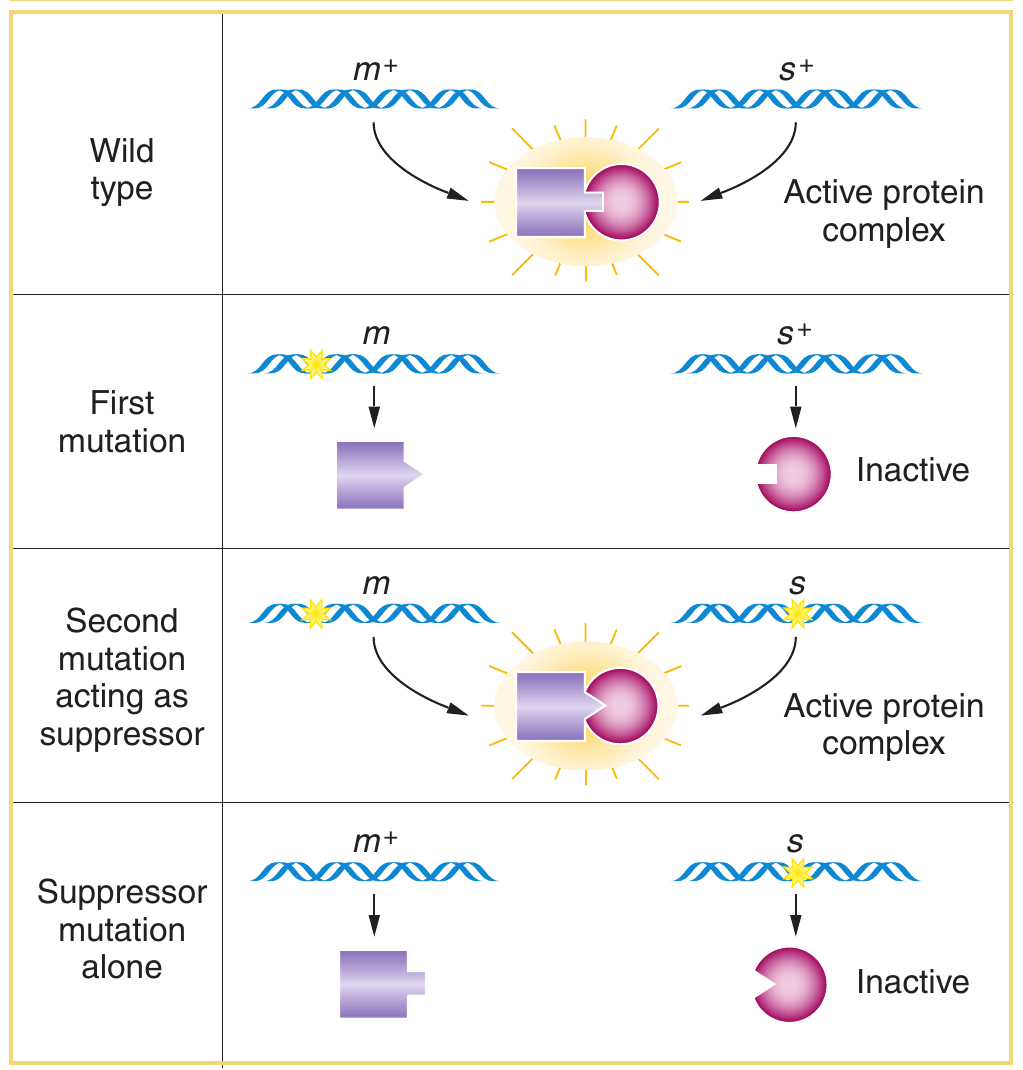
\includegraphics[width=0.4\linewidth]{./../images/molecular_basis_suppression} 

}

\caption{\textbf{Molecular mechanism for suppression.} A first mutation alters the binding site of one protein so that it can no longer bind to a partner. A suppressor mutation in the partner alters the binding site so that both proteins are able to bind once again.}\label{fig:gene-suppression}
\end{figure}
\end{frame}

\begin{frame}{Modifiers}
\protect\hypertarget{modifiers}{}
\begin{itemize}
\tightlist
\item
  Modifier mutation at a second locus changes the degree of expression
  of the mutated gene at the first locus. Regulatory genes are an
  example.
\item
  Regulatory proteins bind to the sequence of the DNA upstream of the
  start site for transcription. These proteins regulate the level of
  transcription.
\item
  As opposed to null mutation of a regulatory gene (in complementation),
  which completely (almost) prevented transcription, some regulatory
  mutations chnage the level of transcription of the target gene so that
  either more (upregulation) or less protein (downregulation) is
  produced.
\item
  A popular downregulating regulatory mutation is that in gene ``B''
  affecting gene A in a fungus such as yeast.
\item
  We cross a leaky mutation \emph{a} with the regulatory mutation b;
\end{itemize}

\[
\textrm{leaky mutant } a.b^+ \times \textrm{inefficient regulator } a^+.b
\]
\end{frame}

\begin{frame}{}
\protect\hypertarget{section-22}{}
\begin{table}

\caption{\label{tab:gene-modifieres}Progency characterization}
\centering
\fontsize{8}{10}\selectfont
\begin{tabular}[t]{ll}
\toprule
Progeny & Phenotype\\
\midrule
$a^+. b^+$ & wild type\\
$a^+.b$ & defective(low trascription)\\
$a.b^+$ & defective (defective protein A)\\
a.b & extremely defective (low transcription of defective protein)\\
\bottomrule
\end{tabular}
\end{table}

\begin{itemize}
\tightlist
\item
  Hence the action of modifiers is seen in the appearance of two grades
  of mutant phenotypes \emph{within} the \(a\) progeny.
\end{itemize}
\end{frame}

\hypertarget{fine-structure-of-gene}{%
\section{Fine structure of gene}\label{fine-structure-of-gene}}

\begin{frame}{}
\protect\hypertarget{section-23}{}
\begin{itemize}
\tightlist
\item
  There are two concepts of gene.

  \begin{itemize}
  \tightlist
  \item
    Older theory aka bead theory
  \item
    Recent theory aka molecular theory
  \end{itemize}
\end{itemize}
\end{frame}

\begin{frame}{Bead theory}
\protect\hypertarget{bead-theory}{}
\begin{itemize}
\tightlist
\item
  A gene is a unit of inheritance.
\item
  Its existence is in the form of an allele.
\item
  Each of the alleles affects a single phenotypic character. All alleles
  map to one chromosome locus.
\item
  A gene gives a mutant phenotype when they are in pairs.
\item
  Genes produce mendelian phenotypic ratio when intercrossed.
\item
  Old concept speaks of indivisible nature of gene (even upon occurance
  of crossing over).
\item
  Crossing over occurs between genes, but crossing over does not occur
  in the same gene. Thus, a gene is fundamental unit of change or
  mutation.
\end{itemize}
\end{frame}

\begin{frame}{}
\protect\hypertarget{section-24}{}
\begin{itemize}
\tightlist
\item
  A gene changes from one allelic form to another. There are no smaller
  units inside the gene that can change.
\item
  A gene is basic unit of function. Parts of a gene if they exist,
  cannot function.
\item
  In the same way as the beads are arranged in an unfastened necklace,
  genes are arranged linearly in a chromosome. So chromosome is a linear
  array of genes according to the bead theory.
\item
  There is no complementation between the allele pair of a gene.
\item
  The old theory of the gene says that there is only one site of
  mutation in a gene. In other words: one gene \textasciitilde{} one
  site of mutation.
\end{itemize}
\end{frame}

\begin{frame}{Molecular theory}
\protect\hypertarget{molecular-theory}{}
\begin{itemize}
\tightlist
\item
  Genes and cistrons are synonymous.
\item
  A cistron or a gene is a fundamental unit to produce a kind of a
  polypeptide.
\item
  But the gene is most commonly used.
\end{itemize}
\end{frame}

\begin{frame}{Complementation test}
\protect\hypertarget{complementation-test}{}
\begin{itemize}
\tightlist
\item
  Determines whether two mutations belong to the same gene.
\item
  Quicker approach when linkage mapping is time consuming.
\item
  The decision whether members of a multiple allelic series are located
  in a single gene or in two or more separately but closely-linked genes
  is based on complementation test.
\item
  When the trans-heterozygotes for two mutant alleles (affecting the
  same trait) have the mutant phenotype, they are placed in the same
  gene. But if they have the wild type phenotype, the mutant alleles are
  considered to be located in two different genes.
\end{itemize}
\end{frame}

\begin{frame}{}
\protect\hypertarget{section-25}{}
\begin{itemize}
\tightlist
\item
  In a diploid, the complementation test is performed by intercrossing
  two individuals that are homozygous for different recessive mutations.
\item
  Next step is to observe whether the progeny have the wild-type
  phenotype. If the progeny are wild type, two recessive mutations must
  be in \emph{different} genes because the respective wild-type alleles
  provide wild-type function. In this case, the two mutations are said
  to have \emph{complemented}.
\item
  Suppose \emph{a1} and \emph{a2} are mutant alleles of two genes.
\item
  Heterozygotes can be represented as follows, depending on whether
  genes are on the same or different chromosomes.
\end{itemize}

\begin{center}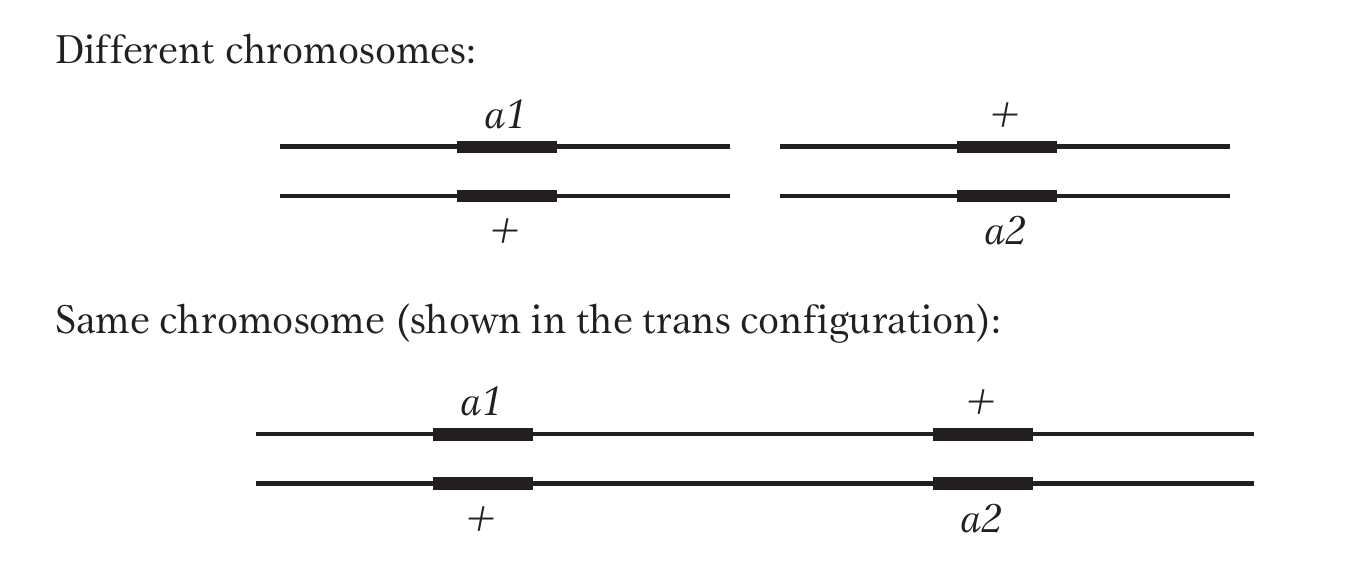
\includegraphics[width=0.35\linewidth]{./../images/gene_location_chromosomes} \end{center}
\end{frame}

\begin{frame}{}
\protect\hypertarget{section-26}{}
\begin{itemize}
\tightlist
\item
  However, if the progeny are not wild type, then the recessive mutant
  must be alleles of the same gene. Because both alleles of the gene are
  mutants, there is no wild-type allele to help distinguish between two
  different mutant alleles of a gene whose wild-type allele is \(a^+\) .
\item
  These alleles could have different mutant sites within the same gene,
  but they would both be non functional.
\item
  The heterozygote \(a^\prime/a^{\prime \prime}\) would be
\end{itemize}

\begin{center}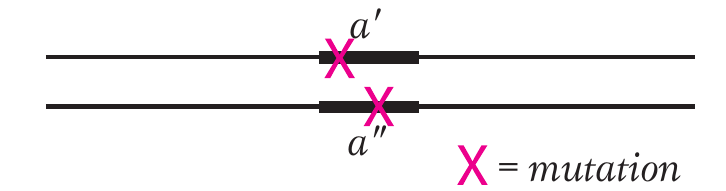
\includegraphics[width=0.35\linewidth]{./../images/gene_location_chromosomes_nc} \end{center}

\begin{itemize}
\tightlist
\item
  At operational level, complementation is defined as the production of
  a wild type phenotype when two haploid genomes bearing different
  recessive mutations are united in the same cell.
\end{itemize}
\end{frame}

\begin{frame}{}
\protect\hypertarget{section-27}{}
\begin{itemize}
\tightlist
\item
  Let us take an example on harebell plants (genus \emph{Campanula}).
  The wild-type flower color of this plant is blue. Let's assume that,
  from a mutant hunt, we have obtained three white-petaled mutants and
  that they are available as homozygous pure-breeding strains.
\item
  They all look the same, and so we do not know whether they are
  genetically identical.
\item
  We will call the mutant strains \(\$\), \(\pounds\), and \(\yen\) to
  avoid any symbolism using letters, which might imply dominance. When
  crossed with wild type, each mutant gives the same results in the
  \(F_1\) and \(F_2\) as follows:
\end{itemize}

\begin{center}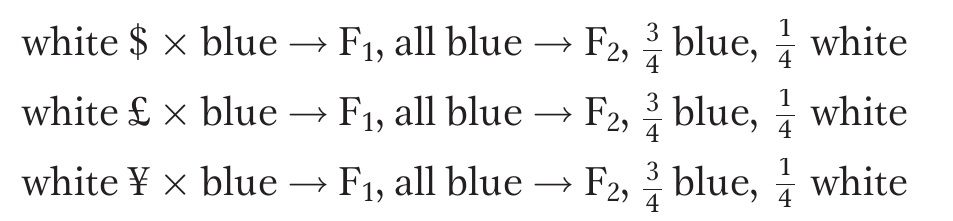
\includegraphics[width=0.35\linewidth]{./../images/gene_complementation_ratios1} \end{center}
\end{frame}

\begin{frame}{}
\protect\hypertarget{section-28}{}
\begin{itemize}
\tightlist
\item
  In each case, results show that the mutant condition is determined by
  the recessive allele of a single gene.
\item
  However, are they three alleles of one gene, of two genes, or of three
  genes?
\item
  Because the mutants are recessive, the question can be answered by the
  complementation test, which asks if the mutants complement one
  another.
\item
  Let us intercross the mutants and assume folloing results are
  obtained:
\end{itemize}

\begin{center}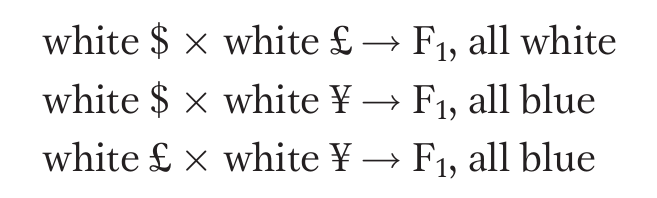
\includegraphics[width=0.35\linewidth]{./../images/gene_complementation_ratios2} \end{center}

\begin{itemize}
\tightlist
\item
  From this set of results, we can conclude that mutants \(\$\) and
  \(\pounds\) must be caused by alleles of one gene (say, \(w1\))
  because they do not complement, but \(\yen\) must be caused by a
  mutant allele of another gene (\(w2\)) because \(\yen\) complements
  both \(\$\) and \(\pounds\).
\end{itemize}
\end{frame}

\begin{frame}{Benzer's experiment on rII locus of T4 with \emph{E.
coli}}
\protect\hypertarget{benzers-experiment-on-rii-locus-of-t4-with-e.-coli}{}
\begin{itemize}
\tightlist
\item
  Because astronomically large numbers of phages can be used in
  phage-recombination analyses, very rare crossover events can be
  detected.
\item
  In the 1950s, Seymour Benzer made use of such rare crossover events to
  map the mutant sites within the rII gene of phage T4, a gene that
  controls lysis.
\item
  For different rII mutant alleles arising spontaneously, the mutant
  site is usually at different positions within the gene.
\item
  Therefore, when two different rII mutants are crossed, a few rare
  crossovers may take place between the mutant sites, producing
  wild-type recombinants, as shown here:
\end{itemize}

\begin{center}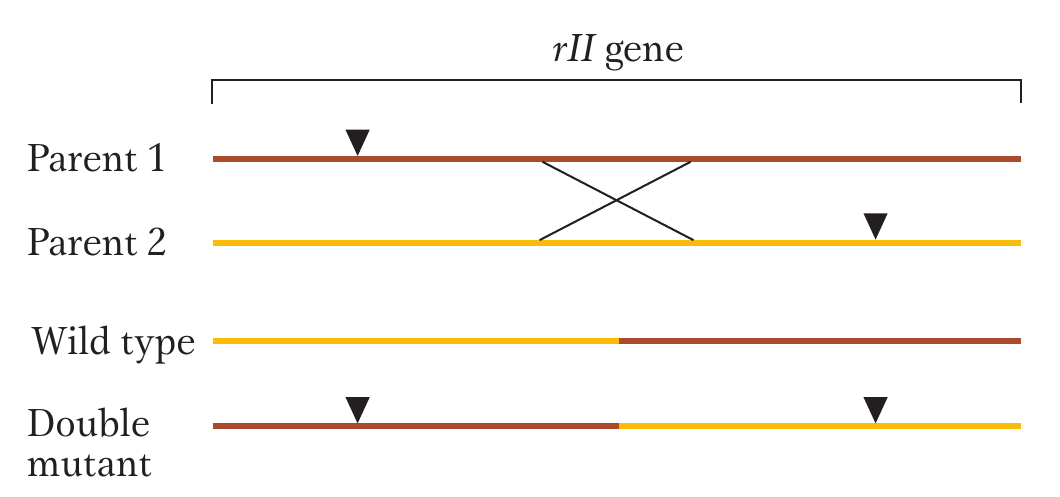
\includegraphics[width=0.35\linewidth]{./../images/phage_recombinants} \end{center}
\end{frame}

\begin{frame}{}
\protect\hypertarget{section-29}{}
As distance between two mutant sites increases, such a crossover event
is more likely. Thus, the frequency of \(rII^+\) recombinants is a
measure of that distance within the gene. (The reciprocal product is a
double mutant and indistinguishable from the parentals.)

Benzer used a clever approach to detect the very rare \(rII^+\)
recombinants. He made use of the fact that rII mutants will not infect a
strain of E. coli called K. Therefore, he made the \(rII\) × \(rII\)
cross on another strain and then plated the phage lysate on a lawn of
strain K. Only \(rII\) + recombinants will form plaques on this lawn.
This way of finding a rare genetic event (in this case, a recombinant)
is a selective system: only the desired rare event can produce a certain
visible outcome.
\end{frame}

\begin{frame}{}
\protect\hypertarget{section-30}{}
\begin{itemize}
\tightlist
\item
  The T4 has A and B cistrons.
\item
  According to Benzer, a gene is a functional unit to produce a
  particular polypeptide.
\item
  Benzer isolated 3000 mutants of rII locus of T4 phage based on
  frequency of crossing over.
\item
  Benzer developed a map of the mutant sites of rII locus of T4 phage.
  The mutation sites were found spread along the entire length of the
  cistron A and B.
\item
  He concluded that crossing over occurs inside the gene or cistron. The
  gene is divisible.
\item
  There are many sites of recombination in a gene. There are many sites
  of change or mutation in a gene.
\item
  A unit of mutation in a gene is a muton. The muton is a single
  nucleotide pair
\item
  Benzer termed sites that are more mutable than other sites as hot
  spots.
\item
  The number of mutational sites was determined to be approximately
  one-fifth (1/5) of the number of nucleotide pairs.
\item
  In other words, the smallest mutable site was five nucleotide pair or
  less.
\end{itemize}
\end{frame}

\begin{frame}{}
\protect\hypertarget{section-31}{}
\begin{itemize}
\tightlist
\item
  From the experiment following conclusions could be drawn:

  \begin{itemize}
  \tightlist
  \item
    A gene is a distinct chromosomal region responsible for a single
    cellular function. It consists of a linear array of potentially
    mutable sites between which recombination can occur.
  \item
    A gene is subdivisible into several units called nucleotide pairs
    (recombination is possible within a gene) among these nucleotide
    pairs.
  \end{itemize}
\end{itemize}
\end{frame}

\hypertarget{bibliography}{%
\section{Bibliography}\label{bibliography}}

\begin{frame}{See also}
\protect\hypertarget{see-also}{}
\begin{itemize}
\tightlist
\item
  For a discourse on types of gene interaction, refer to lecture notes
  on `Introductory genetics', \(3^{rd}\) semester, BScAg.
\end{itemize}
\end{frame}

\begin{frame}{References}
\protect\hypertarget{references}{}
\end{frame}

          \begin{frame}[allowframebreaks]{}
    \bibliographytrue
    \bibliography{./../bibliographies.bib}
    \end{frame}
  


\end{document}
